\documentclass[11pt,oneside]{article}

\usepackage[a4paper,margin=27mm,headheight=15pt]{geometry}
\usepackage[T1]{fontenc}
\usepackage[utf8]{inputenc}
\IfFileExists{libertinus.sty}{\usepackage{libertinus}}{\usepackage{lmodern}}
\usepackage{microtype}
\usepackage{amsmath,amssymb,amsthm,mathtools,mathrsfs}
\usepackage{bm}
% Canonical mathematical notation for active FabiusFunction LaTeX documents.
%
% This file is intentionally a plain TeX input rather than a LaTeX package.
% Every standalone document loads it by an explicit path relative to that
% document's directory; included fragments inherit the definitions from their
% root document.  Keep this file independent of document layout and metadata.
%
% Contract:
%   * one command has one mathematical meaning throughout the active corpus;
%   * names encode semantic roles rather than a document-local choice of letter;
%   * visually similar but differently normalized objects have different print;
%   * every command below is defined normatively in the notation catalogue.
%
% The active corpus excludes docs/archive/.  Historical sources may retain
% their original notation only inside an explicitly labelled quotation.

\makeatletter
\@ifundefined{mathbb}{%
  \PackageError{fabius-notation}{The amssymb package must be loaded first}%
    {Load amsmath and amssymb before inputting fabius-notation.tex.}%
}{}
\@ifundefined{operatorname}{%
  \PackageError{fabius-notation}{The amsmath package must be loaded first}%
    {Load amsmath before inputting fabius-notation.tex.}%
}{}
\makeatother

% Version stamp used by the catalogue and by static audits.
\newcommand{\FabiusNotationVersion}{2026-08-31}

% Number systems.  NaturalNumbers is explicitly the nonnegative convention.
\newcommand{\NaturalNumbers}{\mathbb{N}_{0}}
\newcommand{\PositiveIntegers}{\mathbb{N}_{>0}}
\newcommand{\IntegerNumbers}{\mathbb{Z}}
\newcommand{\RationalNumbers}{\mathbb{Q}}
\newcommand{\RealNumbers}{\mathbb{R}}
\newcommand{\ComplexNumbers}{\mathbb{C}}
\newcommand{\ExtendedRealNumbers}{\overline{\mathbb{R}}}

% The three principal Fabius--Rvachev functions.  Subscripts are deliberate:
% a bare F and a calligraphic F have several unrelated uses in the corpus.
\newcommand{\FabiusBounded}{F_{\mathrm{bd}}}
\newcommand{\FabiusGlobal}{F_{\mathrm{gl}}}
\newcommand{\FabiusQuantile}{Q_{F}}
\newcommand{\FabiusClampedQuantile}{Q_{F,\mathrm{cl}}}
\newcommand{\RvachevUp}{\operatorname{up}}

% Constants, elementary operators, and delimiters.
\newcommand{\EulerE}{\mathrm{e}}
\newcommand{\ImaginaryUnit}{\mathrm{i}}
\newcommand{\Differential}{\mathop{}\!\mathrm{d}}
\newcommand{\AbsoluteValue}[1]{\left\lvert #1\right\rvert}
\newcommand{\Norm}[1]{\left\lVert #1\right\rVert}
\newcommand{\Floor}[1]{\left\lfloor #1\right\rfloor}
\newcommand{\Ceiling}[1]{\left\lceil #1\right\rceil}
\newcommand{\FractionalPart}[1]{\left\{#1\right\}}
\newcommand{\PositivePart}[1]{\left(#1\right)_{+}}
\newcommand{\IndicatorOf}[1]{\mathbf{1}_{#1}}
\newcommand{\SetOf}[1]{\left\{#1\right\}}
\newcommand{\InnerProduct}[1]{\left\langle #1\right\rangle}
\newcommand{\CardinalityOf}[1]{\left\lvert #1\right\rvert}
\newcommand{\DefinitionEquals}{\mathrel{\coloneqq}}
\newcommand{\Sign}{\operatorname{sgn}}
\newcommand{\IdentityOperator}{\operatorname{id}}
\newcommand{\SpanOperator}{\operatorname{span}}
\newcommand{\TraceOperator}{\operatorname{tr}}
\newcommand{\RankOperator}{\operatorname{rank}}
\newcommand{\DiagonalOperator}{\operatorname{diag}}
\newcommand{\ResidueOperator}{\operatorname*{Res}}
\newcommand{\LeastCommonMultiple}{\operatorname{lcm}}
\newcommand{\OrderOperator}{\operatorname{ord}}
\newcommand{\PrincipalLogarithm}{\operatorname{Log}}
\newcommand{\FallingFactorial}[2]{\left(#1\right)^{\underline{#2}}}
\newcommand{\RisingFactorial}[2]{\left(#1\right)^{\overline{#2}}}

% Support, topology, convolution, and metric notation.
\newcommand{\SupportOperator}{\operatorname{supp}}
\newcommand{\SupportOf}[1]{\SupportOperator\!\left(#1\right)}
\newcommand{\TopologicalSupportOf}[1]{\operatorname{tsupp}\!\left(#1\right)}
\newcommand{\Convolution}{\mathbin{*}}
\newcommand{\MetricDistance}{\operatorname{dist}}
\newcommand{\TotalVariationDistance}{d_{\mathrm{TV}}}

% Probability.  Equality and convergence in law are not metric distance.
\newcommand{\Probability}{\mathbb{P}}
\newcommand{\Expectation}{\mathbb{E}}
\newcommand{\Variance}{\operatorname{Var}}
\newcommand{\Covariance}{\operatorname{Cov}}
\newcommand{\LawOperator}{\operatorname{Law}}
\newcommand{\LawOf}[1]{\LawOperator\!\left(#1\right)}
\newcommand{\EqualInLaw}{\mathrel{\overset{\mathrm{law}}{=}}}
\newcommand{\ConvergesInLaw}{\mathrel{\xrightarrow{\mathrm{law}}}}

% Fourier and integral transforms.  The printed labels expose normalization.
% FourierTwoPi uses exp(-2*pi*i*x*xi); FourierAngular uses exp(-i*x*omega).
\newcommand{\FourierTwoPi}[1]{\widehat{#1}_{\,2\pi}}
\newcommand{\FourierAngular}[1]{\widehat{#1}_{\,\mathrm{ang}}}
\newcommand{\LaplaceTransformSymbol}{\mathcal{L}}
\newcommand{\MellinTransformSymbol}{\mathcal{M}}
\newcommand{\LaplaceTransformOf}[1]{\LaplaceTransformSymbol\!\left[#1\right]}
\newcommand{\MellinTransformOf}[1]{\MellinTransformSymbol\!\left[#1\right]}
\newcommand{\MomentGeneratingFunction}[1]{M_{#1}}
\newcommand{\CharacteristicFunction}[1]{\varphi_{#1}}

% The two standard sinc functions must never share one symbol.
\newcommand{\SincRad}{\operatorname{sinc}_{\mathrm{rad}}}
\newcommand{\SincPi}{\operatorname{sinc}_{\pi}}

% Binary arithmetic and Thue--Morse notation.
\newcommand{\BinaryDigitSum}{\operatorname{wt}_{2}}
\newcommand{\ThueMorseSignSymbol}{\varepsilon}
\newcommand{\ThueMorseSign}[1]{\varepsilon_{#1}}
\newcommand{\PadicValuation}[1]{\nu_{#1}}
\newcommand{\TwoAdicValuation}{\nu_{2}}

% q-series notation.  Every base is an explicit argument.
\newcommand{\QPochhammer}[3]{\left(#1;#2\right)_{#3}}
\newcommand{\GaussianBinomial}[3]{%
  \genfrac{[}{]}{0pt}{}{#1}{#2}_{#3}%
}
\newcommand{\QInteger}[2]{\left[#1\right]_{#2}}

% Named special functions.
\newcommand{\Polylogarithm}{\operatorname{Li}}
\newcommand{\LambertW}{W}
\newcommand{\GammaFunction}{\Gamma}
\newcommand{\RiemannZeta}{\zeta}

% Asymptotics.  BigO and LittleO are operator tokens for existing formula
% grammar; prefer the At forms so that the limiting regime is printed.
\newcommand{\BigO}{\mathcal{O}}
\newcommand{\LittleO}{o}
\newcommand{\BigOAt}[2]{\mathcal{O}_{#2}\!\left(#1\right)}
\newcommand{\LittleOAt}[2]{o_{#2}\!\left(#1\right)}

\usepackage{booktabs,longtable,array,tabularx}
\usepackage{graphicx}
\usepackage{pgfplots}
\usepackage{xcolor}
\usepackage{enumitem}
\usepackage{fancyhdr}
\usepackage{titlesec}
\usepackage{listings}
\usepackage{xurl}
\usepackage{hyperref}
\usepackage[nameinlink,noabbrev]{cleveref}
\usepackage{aliascnt}

\definecolor{linkblue}{RGB}{25,75,135}
\definecolor{shadegray}{RGB}{246,247,249}
\definecolor{rulegray}{RGB}{195,201,208}
\pgfplotsset{compat=1.18}

\hypersetup{
  colorlinks=true,
  linkcolor=linkblue,
  citecolor=linkblue,
  urlcolor=linkblue,
  pdftitle={Interpolation on a Geometric Comb},
  pdfauthor={Research report for the ProveIt Fabius Function project},
  pdfsubject={Geometric-comb interpolation, Jackson calculus, modal filters, B-splines, and Fabius--Rvachev connections},
  pdfkeywords={geometric interpolation, q-binomial, Jackson derivative, Fabius function, Rvachev up-function}
}

\pagestyle{fancy}
\fancyhf{}
\fancyhead[L]{\small Interpolation on a geometric comb}
\fancyhead[R]{\small\nouppercase{\leftmark}}
\fancyfoot[C]{\thepage}
\renewcommand{\headrulewidth}{0.4pt}

\titleformat{\section}{\Large\bfseries}{\thesection}{0.7em}{}
\titleformat{\subsection}{\large\bfseries}{\thesubsection}{0.7em}{}
\titleformat{\subsubsection}{\normalsize\bfseries}{\thesubsubsection}{0.7em}{}
\setcounter{secnumdepth}{3}
\numberwithin{equation}{section}
\setcounter{tocdepth}{2}
\setlist[itemize]{leftmargin=2em,itemsep=0.25em,topsep=0.4em}
\setlist[enumerate]{leftmargin=2.3em,itemsep=0.25em,topsep=0.4em}
\setlength{\emergencystretch}{2em}

\newtheorem{theorem}{Theorem}[section]

\newaliascnt{proposition}{theorem}
\newtheorem{proposition}[proposition]{Proposition}
\aliascntresetthe{proposition}
\newaliascnt{lemma}{theorem}
\newtheorem{lemma}[lemma]{Lemma}
\aliascntresetthe{lemma}
\newaliascnt{corollary}{theorem}
\newtheorem{corollary}[corollary]{Corollary}
\aliascntresetthe{corollary}
\newaliascnt{conjecture}{theorem}
\newtheorem{conjecture}[conjecture]{Conjecture}
\aliascntresetthe{conjecture}
\newaliascnt{problem}{theorem}
\newtheorem{problem}[problem]{Problem}
\aliascntresetthe{problem}
\theoremstyle{definition}
\newaliascnt{definition}{theorem}
\newtheorem{definition}[definition]{Definition}
\aliascntresetthe{definition}
\newaliascnt{example}{theorem}
\newtheorem{example}[example]{Example}
\aliascntresetthe{example}
\newaliascnt{algorithm}{theorem}
\newtheorem{algorithm}[algorithm]{Algorithm}
\aliascntresetthe{algorithm}
\theoremstyle{remark}
\newaliascnt{remark}{theorem}
\newtheorem{remark}[remark]{Remark}
\aliascntresetthe{remark}

\crefname{proposition}{proposition}{propositions}
\Crefname{proposition}{Proposition}{Propositions}
\crefname{lemma}{lemma}{lemmas}
\Crefname{lemma}{Lemma}{Lemmas}
\crefname{corollary}{corollary}{corollaries}
\Crefname{corollary}{Corollary}{Corollaries}
\crefname{conjecture}{conjecture}{conjectures}
\Crefname{conjecture}{Conjecture}{Conjectures}
\crefname{problem}{problem}{problems}
\Crefname{problem}{Problem}{Problems}
\crefname{definition}{definition}{definitions}
\Crefname{definition}{Definition}{Definitions}
\crefname{example}{example}{examples}
\Crefname{example}{Example}{Examples}
\crefname{algorithm}{algorithm}{algorithms}
\Crefname{algorithm}{Algorithm}{Algorithms}
\crefname{remark}{remark}{remarks}
\Crefname{remark}{Remark}{Remarks}

\newenvironment{statusbox}[1]{%
  \par\smallskip\noindent\begin{center}\begin{minipage}{0.94\textwidth}%
  \color{black}\hrule\vspace{0.6em}\small\textbf{#1}\par\smallskip
}{%
  \vspace{0.6em}\hrule\end{minipage}\end{center}\smallskip
}

\newcommand{\Gc}{\mathcal G}
\newcommand{\Rc}{\mathcal R}
\newcommand{\Ic}{\mathcal I}
\newcommand{\Dc}{\mathcal D}
\newcommand{\Cc}{\mathcal C}
\newcommand{\Bc}{\mathcal B}
\newcommand{\Thetaop}{\Theta}

\title{\textbf{Interpolation on a Geometric Comb}\\[0.45em]
\large Lagrange and Newton Formulas, Jackson Calculus, Modal Filters,\\
Geometric B-Splines, and Fabius--Rvachev Connections}
\author{Research report for the ProveIt Fabius Function project}
\date{30 August 2026}

\begin{document}
\maketitle

\begin{abstract}
Let $0<q<1$ and let
\[
  \Cc(A,q)=\{A,Aq,Aq^2,\ldots\}
\]
be a geometric comb accumulating at the origin.  The linked ProveIt monograph
already develops the finite Lagrange row that extrapolates polynomial data on
$1,q,\ldots,q^n$ to $0$, its Gaussian-binomial moment cancellations, and its
application to scaled Fourier samples of the Rvachev function.  This report
builds a more systematic interpolation theory around that row and derives a
number of extensions that do not merely repeat the existing formulas.

The main results include: explicit scale-covariant barycentric and Newton
formulas on $Aq^k$; an exact identification of Newton divided differences with
Jackson derivatives; a locally uniformly convergent infinite Newton series for
analytic functions; a sharp coefficient-majorant error bound summed by the
reciprocal $q$-binomial theorem; a dilation-operator factorization and an
$O(n^2)$ triangular algorithm; unique confluent filters annihilating prescribed
Puiseux--logarithmic modes; exact total variation and its modular $q\uparrow1$
asymptotic; an $\ell^1$ boundary-layer limit and a regular-variation theorem;
a Hermite--Genocchi remainder represented by a positive geometric-knot
B-spline; explicit moments and a scaling limit of that B-spline to a positive
random variable whose Laplace transform is $1/(-s;q)_\infty$; finite box-spline
approximants to geometric-uniform laws and their Thue--Morse collapse at
$q=1/2$; an exact sign formula and probabilistic remainder identity for Fabius
values near the flat endpoint; and a base-squaring principle explaining why the
Rvachev Fourier problem naturally uses interpolation base $Q=q^2$.

All statements advertised as theorems have manuscript proofs.  Conjectures and
open problems are separated explicitly.  A commented Python program reproduces
the numerical checks and figures and is included with the source and rendered
PDF.  Manuscript proof, numerical replay, and Lean proof status are distinct.
\end{abstract}

\begin{statusbox}{Result and formalization status}
The finite Gaussian-comb core has substantial, independently checked Lean
coverage.  In particular,
\nolinkurl{GeometricLagrangeQMoments.lean} contains the natural-moment residual
and finite row-variation identities,
\nolinkurl{LimitConditionNumber.lean} proves convergence of the finite
condition numbers to the infinite $q$-product,
\nolinkurl{GeometricUniformLaw.lean} and
\nolinkurl{GeometricUniformCDF.lean} construct the geometric-uniform law and
its smooth CDF/density, and \nolinkurl{RvachevQBinomialFilter.lean} contains a
finite Gaussian transform for the Rvachev Fourier product.  Those modules do
not make this whole report Lean-proved.  No exact current theorem was located
for the Jackson divided-difference identification, locally uniform infinite
Newton reconstruction, confluent Puiseux--log filters, regular-variation
transfer, Hermite--Genocchi/B-spline probability law, perpetuity scaling limit,
Fabius boundary expectation, or entire scale reconstruction.  Those results,
the two conjectures, and the five numbered research problems remain manuscript
mathematics.  The companion computations are diagnostics, not proof premises.
\end{statusbox}

\vspace{0.5em}
\noindent\textbf{Scope and priority.}
The report was written after inspecting the linked ProveIt monograph and the
nearby primary Fabius/Rvachev exposition in the same repository.  ``New'' below
means new relative to those inspected documents; it is not a claim that every
result is absent from the wider literature.  Classical ingredients such as
Newton interpolation, Hermite--Genocchi formulas, regular variation, and
B-splines are cited where they enter.

\tableofcontents
\newpage

\section{Introduction and contribution map}

\subsection{Why a geometric comb is different}

Classical interpolation is often organized around equally spaced nodes,
Chebyshev nodes, or a fixed compact array.  A geometric comb has a different
geometry.  Its nodes accumulate inside the domain, the local mesh ratio is
constant rather than the mesh difference, and the dilation operator
$f(x)\mapsto f(qx)$ diagonalizes the monomials.  Consequently the natural
algebra is not ordinary finite-difference algebra but Gaussian-binomial and
Jackson $q$-calculus.

The accumulation point makes the problem look ill conditioned: the full
Vandermonde determinant tends to zero extremely rapidly.  Yet the particular
linear functional ``evaluate at the accumulation point'' has a bounded total
variation for every fixed $q<1$, uniformly in the interpolation order.  This
apparent paradox is one of the central themes of the report.  Coefficient
recovery in the monomial basis is badly conditioned, while the scale-adapted
functional is stable because its weights develop a universal boundary layer at
the smallest nodes.

The same algebra also occurs in the Fabius/Rvachev setting.  The Fabius random
variable is an infinite sum of geometrically weighted uniforms; the Rvachev
Fourier transform is an infinite product of sinc factors; and scaled Fourier
samples of an even function convert the physical scale ratio into its square.
Thus interpolation, $q$-series, probability, compactly supported splines, and
self-similar smooth functions are not separate topics here.  They are different
representations of the same dilation structure.

\subsection{Baseline from the linked monograph}

The source monograph \cite{ProveItMonograph} already contains the following
core facts, which are treated here as a baseline rather than as new results:
\begin{enumerate}[label=(\roman*),leftmargin=2em]
\item Newton interpolation on $1,q,\ldots,q^n$ with explicit coefficients;
\item the reversed Gaussian row
\[
  N_{n,k}=(-1)^{n-k}q^{\binom{n-k+1}{2}}\GaussianBinomial{n}{k}{q};
\]
\item the normalized origin weights
\[
  \lambda_{n,k}^{(q)}=
  \frac{(-1)^{n-k}q^{\binom{n-k+1}{2}}}
       {(q;q)_k(q;q)_{n-k}};
\]
\item exact annihilation of the powers $q^{kd}$ for $1\le d\le n$ and the
Gaussian residual for $d\ge n+1$;
\item formal and analytic filters obtained from these moments;
\item geometric-uniform random sums, the Fabius function at $q=1/2$, and a
finite Fourier filter for the Rvachev sinc product.
\end{enumerate}
The present report retains this notation but develops the surrounding theory in
a form suited to reuse, asymptotics, and future formalization.

\subsection{Results developed here}

The principal additions are organized as follows.
\begin{longtable}{p{0.23\textwidth}p{0.70\textwidth}}
\toprule
Topic & Result developed in this report\\
\midrule
\endhead
Comb geometry & Exact Vandermonde determinant for $Aq^k$, scale covariance,
and barycentric denominators.\\
Newton theory & Jackson-derivative identification, two inverse Gaussian basis
transforms, and a convergent infinite Newton expansion for analytic functions.\\
Analytic error & Exact Taylor tail and the sharper bound
$q^{\binom{n+1}{2}}t^{n+1}/(t;q)_{n+1}$.\\
Operator theory & Spectral polynomial in the dilation operator, recursive
factorization, and unique filters for arbitrary simple or confluent modes.\\
Asymptotics & Exact total variation, $q\uparrow1$ modular growth, an $\ell^1$
boundary layer, and a theorem for regularly varying germs.\\
Smooth remainder & Hermite--Genocchi expectation, sign theorem, positive
geometric-knot B-spline density, and exact Gaussian-binomial moments.\\
Scaling limit & Rescaled geometric B-splines converge weakly to
$Z_q=\sum_{j\ge0}q^jE_j$ with Laplace transform $1/(-s;q)_\infty$ and an
explicit exponential series for its density.\\
Fabius function & Exact boundary-comb identity, alternating sign, factorial
bound, and a Dirichlet-average interpretation of exact dyadic filters.\\
Rvachev function & Base-squaring principle $Q=c^2$, entire Newton
reconstruction from multiscale samples, and moment-flat residuals.\\
\bottomrule
\end{longtable}

\section{Notation and elementary $q$-identities}

Throughout the main body, $0<q<1$, $A>0$, and $n\in\NaturalNumbers$.  Most algebraic
formulas remain valid for complex $A\ne0$ and $0<|q|<1$ after the obvious
noncollision assumptions.

\begin{definition}[$q$-shifted factorial and Gaussian coefficient]
For $m\in\NaturalNumbers$,
\[
 (a;q)_m:=\prod_{j=0}^{m-1}(1-aq^j),\qquad
 (a;q)_\infty:=\prod_{j=0}^{\infty}(1-aq^j),
\]
and
\[
 \GaussianBinomial{m}{k}{q}:=\frac{(q;q)_m}{(q;q)_k(q;q)_{m-k}}
 \quad(0\le k\le m).
\]
We also write
\[
 [m]_q:=\frac{1-q^m}{1-q},\qquad
 [m]_q!:=\prod_{j=1}^m[j]_q=\frac{(q;q)_m}{(1-q)^m}.
\]
\end{definition}

We repeatedly use the finite and reciprocal $q$-binomial theorems
\begin{align}
 (z;q)_m
 &=\sum_{k=0}^m(-1)^kq^{\binom{k}{2}}\GaussianBinomial{m}{k}{q} z^k,
 \label{eq:finite-q-binomial}\\
 \frac1{(z;q)_{m+1}}
 &=\sum_{r=0}^{\infty}\GaussianBinomial{m+r}{m}{q}z^r,
 \qquad |z|<1.
 \label{eq:reciprocal-q-binomial}
\end{align}
These are standard; see DLMF Chapter 17 \cite{DLMF17} or
Gasper--Rahman \cite{GasperRahman}.

Let $h_r(y_0,\ldots,y_m)$ denote the complete homogeneous symmetric
polynomial, characterized by
\[
 \sum_{r\ge0}h_r(y_0,\ldots,y_m)t^r
 =\prod_{j=0}^m\frac1{1-y_jt}.
\]
A direct use of \eqref{eq:reciprocal-q-binomial} gives
\begin{equation}
 h_r(A,Aq,\ldots,Aq^m)=A^r\GaussianBinomial{m+r}{m}{q}.
 \label{eq:h-geometric}
\end{equation}
This small identity is the source of nearly every Gaussian residual below.

\section{Geometry of the comb}

\begin{definition}[Geometric comb]
For $A\ne0$ and $0<|q|<1$, define
\[
 \Cc(A,q):=\{Aq^k:k\in\NaturalNumbers\},\qquad
 \Cc_n(A,q):=\{A,Aq,\ldots,Aq^n\}.
\]
A shifted comb $\{aq^{s+k}:k\ge0\}$ is the same object with $A=aq^s$.
\end{definition}

\subsection{Scale covariance}

If $x=A\tau$, every Lagrange cardinal polynomial on $\Cc_n(A,q)$ is a
function only of $(\tau,q)$.  Thus the scale $A$ is not an essential parameter;
it simply transports the theory between neighborhoods of the origin.

\begin{proposition}[Scale covariance]
Let $\ell_{n,k}^{A,q}$ be the cardinal polynomial for the node $Aq^k$.
Then
\[
 \ell_{n,k}^{A,q}(A\tau)=\ell_{n,k}^{1,q}(\tau).
\]
In particular, the weights for evaluation at $0$ are independent of $A$ and of
the shift exponent $s$.
\end{proposition}

\begin{proof}
In the product
\[
 \ell_{n,k}^{A,q}(A\tau)
 =\prod_{\substack{0\le j\le n\\j\ne k}}
   \frac{A\tau-Aq^j}{Aq^k-Aq^j},
\]
each factor $A$ cancels.
\end{proof}

\subsection{Vandermonde determinant}

The global monomial-basis interpolation problem becomes rapidly singular.
The exact determinant quantifies the effect.

\begin{theorem}[Geometric Vandermonde determinant]
Let $V_n=(x_i^j)_{0\le i,j\le n}$ with $x_i=Aq^i$, and put
$N=\binom{n+1}{2}$.  Then
\begin{equation}
 \det V_n
 =(-1)^N A^N q^{\binom{n+1}{3}}
   \prod_{d=1}^n(1-q^d)^{n+1-d}.
 \label{eq:vandermonde}
\end{equation}
\end{theorem}

\begin{proof}
The usual Vandermonde product gives
\[
 \det V_n=\prod_{0\le i<j\le n}(Aq^j-Aq^i).
\]
For each pair,
$Aq^j-Aq^i=-Aq^i(1-q^{j-i})$.  There are $N$ pairs.  Moreover
\[
 \sum_{0\le i<j\le n}i
 =\sum_{i=0}^{n-1}i(n-i)=\binom{n+1}{3},
\]
and a fixed difference $d=j-i$ occurs $n+1-d$ times.  Multiplication yields
\eqref{eq:vandermonde}.
\end{proof}

\begin{remark}[Conditioning is functional-dependent]
The factor $q^{\binom{n+1}{3}}$ makes the determinant extremely small.  It
would be a mistake, however, to infer that every linear functional of the
interpolant is comparably unstable.  The origin functional has total variation
bounded by $(-q;q)_\infty/(q;q)_\infty$ for fixed $q$; see
\cref{sec:stability}.  The monomial coefficients are ill conditioned, while a
scale-adapted extrapolated value need not be.
\end{remark}

\section{Lagrange interpolation on a finite comb}

\subsection{Cardinal functions and barycentric weights}

Define the node polynomial
\[
 \omega_{n,A,q}(x):=\prod_{j=0}^n(x-Aq^j)
 =x^{n+1}(A/x;q)_{n+1},
\]
where the last expression is interpreted by polynomial continuation at $x=0$.

\begin{theorem}[Explicit denominator and cardinal function]
For $0\le k\le n$,
\begin{equation}
 d_{n,k}^{A,q}:=\prod_{\substack{0\le j\le n\\j\ne k}}
 (Aq^k-Aq^j)
 =(-1)^kA^nq^{kn-k(k+1)/2}(q;q)_k(q;q)_{n-k}.
 \label{eq:bary-denominator}
\end{equation}
Consequently
\begin{equation}
 \ell_{n,k}^{A,q}(x)
 =\frac{\omega_{n,A,q}(x)}{(x-Aq^k)d_{n,k}^{A,q}},
 \label{eq:cardinal-omega}
\end{equation}
with the removable value $1$ at $x=Aq^k$.
\end{theorem}

\begin{proof}
For $j<k$,
\[
 Aq^k-Aq^j=-Aq^j(1-q^{k-j}),
\]
whose product is
$(-1)^kA^kq^{k(k-1)/2}(q;q)_k$.  For $j>k$ the product is
$A^{n-k}q^{k(n-k)}(q;q)_{n-k}$.  Multiplying gives
\eqref{eq:bary-denominator}; \eqref{eq:cardinal-omega} is the standard
cardinal formula.
\end{proof}

The first-form barycentric weights are $b_{n,k}^{A,q}=1/d_{n,k}^{A,q}$.  For
$x$ not equal to a node, the interpolant of data $y_k$ can therefore be
computed as
\begin{equation}
 \Ic_n y(x)=
 \frac{\displaystyle\sum_{k=0}^n\frac{b_{n,k}^{A,q}y_k}{x-Aq^k}}
      {\displaystyle\sum_{k=0}^n\frac{b_{n,k}^{A,q}}{x-Aq^k}}.
 \label{eq:barycentric-second}
\end{equation}
This avoids solving the Vandermonde system and is the recommended formula away
from the accumulation point.

\subsection{The origin row}

\begin{corollary}[Scale-free origin weights]
For polynomial data of degree at most $n$,
\[
 p(0)=\sum_{k=0}^n\lambda_{n,k}^{(q)}p(Aq^k),
\]
where
\begin{equation}
 \lambda_{n,k}^{(q)}
 =\ell_{n,k}^{A,q}(0)
 =\frac{(-1)^{n-k}q^{\binom{n-k+1}{2}}}
 {(q;q)_k(q;q)_{n-k}}.
 \label{eq:lambda}
\end{equation}
Equivalently,
\begin{equation}
 \sum_{k=0}^n\lambda_{n,k}^{(q)}z^k
 =W_{n,q}(z):=\frac{\prod_{j=1}^n(z-q^j)}{(q;q)_n}.
 \label{eq:row-polynomial}
\end{equation}
\end{corollary}

\begin{proof}
Set $x=0$ in the product definition of the cardinal function and simplify with
\eqref{eq:bary-denominator}.  Formula \eqref{eq:row-polynomial} follows from
the finite $q$-binomial theorem or by observing that both sides are degree-$n$
polynomials with the same roots and value $1$ at $z=1$.
\end{proof}

\subsection{Residuals at an arbitrary target}

The usual interpolation remainder becomes especially explicit on a geometric
comb.

\begin{theorem}[Complete-homogeneous residual]
Let $r\ge0$.  Interpolation of the monomial $u^{n+1+r}$ at
$A,Aq,\ldots,Aq^n$, evaluated at $x$, satisfies
\begin{align}
 \sum_{k=0}^n\ell_{n,k}^{A,q}(x)(Aq^k)^{n+1+r}
 &=x^{n+1+r}-\omega_{n,A,q}(x)
   h_r(x,A,Aq,\ldots,Aq^n)\notag\\
 &=x^{n+1+r}-\omega_{n,A,q}(x)
   \sum_{j=0}^r x^jA^{r-j}\GaussianBinomial{n+r-j}{n}{q}.
 \label{eq:arbitrary-residual}
\end{align}
\end{theorem}

\begin{proof}
For a monomial of degree $n+1+r$, the divided difference of order $n+1$ at
$x,A,Aq,\ldots,Aq^n$ is the complete homogeneous polynomial
$h_r(x,A,Aq,\ldots,Aq^n)$.  The standard remainder identity is therefore the
first line.  Splitting a complete homogeneous polynomial according to the
power of the distinguished variable $x$ and using \eqref{eq:h-geometric}
gives the second line.
\end{proof}

At $x=0$ this gives the exact moment row.

\begin{corollary}[All origin moments]
For $d\in\NaturalNumbers$,
\begin{equation}
 \sum_{k=0}^n\lambda_{n,k}^{(q)}(Aq^k)^d
 =\begin{cases}
  1,&d=0,\\
  0,&1\le d\le n,\\
  (-1)^nA^dq^{\binom{n+1}{2}}
  \GaussianBinomial{d-1}{n}{q},&d\ge n+1.
 \end{cases}
 \label{eq:all-moments}
\end{equation}
\end{corollary}

\subsection{Exact analytic tail and a sharp majorant}

For a formal or convergent power series $f(x)=\sum_{m\ge0}a_mx^m$, define
\begin{equation}
 (\Gc_{n,q}f)(A):=\sum_{k=0}^n\lambda_{n,k}^{(q)}f(Aq^k).
 \label{eq:G-definition}
\end{equation}
Then \eqref{eq:all-moments} gives the exact identity
\begin{equation}
 (\Gc_{n,q}f)(A)-f(0)
 =(-1)^nq^{\binom{n+1}{2}}
  \sum_{r=0}^{\infty}\GaussianBinomial{n+r}{n}{q}a_{n+1+r}A^{n+1+r}.
 \label{eq:exact-analytic-tail}
\end{equation}

\begin{theorem}[Reciprocal-$q$-binomial majorant]
Suppose $f$ is analytic in $|z|<R$ and its Taylor coefficients satisfy
$|a_m|\le MR^{-m}$.  Put $t=|A|/R<1$.  Then
\begin{equation}
 \left|(\Gc_{n,q}f)(A)-f(0)\right|
 \le M q^{\binom{n+1}{2}}
 \frac{t^{n+1}}{(t;q)_{n+1}}.
 \label{eq:sharp-majorant}
\end{equation}
The right side is coefficientwise sharp: equality in the majorant sum is
attained when the relevant coefficients have a common phase and magnitude
$MR^{-m}$.
\end{theorem}

\begin{proof}
Take absolute values in \eqref{eq:exact-analytic-tail} and apply
\eqref{eq:reciprocal-q-binomial}:
\[
 \sum_{r\ge0}\GaussianBinomial{n+r}{n}{q}t^r=\frac1{(t;q)_{n+1}}.
\]
\end{proof}

For fixed $q<1$ and $t<1$, $(t;q)_{n+1}$ tends to the positive constant
$(t;q)_\infty$.  Thus the dominant convergence factor is the
supergeometric $q^{n(n+1)/2}$, multiplied by the ordinary $t^{n+1}$.

\section{Newton interpolation and Jackson calculus}

\subsection{Jackson derivative as a divided difference}

Define the Jackson derivative
\begin{equation}
 (D_qf)(x):=\frac{f(x)-f(qx)}{(1-q)x},\qquad x\ne0.
 \label{eq:Jackson}
\end{equation}
For analytic $f$, the value at $x=0$ is supplied by continuity.

\begin{theorem}[Geometric divided differences]
For every polynomial $f$ and $k\ge0$,
\begin{equation}
 f[A,Aq,\ldots,Aq^k]=\frac{D_q^kf(A)}{[k]_q!}.
 \label{eq:divdiff-Jackson}
\end{equation}
The identity extends to analytic $f$ wherever the divided difference is
defined.
\end{theorem}

\begin{proof}
Both sides are linear in $f$, so it suffices to take $f(x)=x^m$.  If $m<k$,
both sides vanish.  If $m=k+r$, the divided difference is
\[
 h_r(A,Aq,\ldots,Aq^k)=A^r\GaussianBinomial{k+r}{k}{q}.
\]
On the other hand,
\[
 D_q^kx^{k+r}\big|_{x=A}
 =[k+r]_q[k+r-1]_q\cdots[r+1]_qA^r,
\]
and division by $[k]_q!$ gives the same Gaussian coefficient.
\end{proof}

\subsection{Newton formula and explicit coefficients}

\begin{theorem}[Newton--Jackson interpolation]
The degree-$n$ interpolant of $f$ on $A,Aq,\ldots,Aq^n$ is
\begin{equation}
 \Ic_nf(x)=\sum_{k=0}^n
 \frac{D_q^kf(A)}{[k]_q!}
 \prod_{r=0}^{k-1}(x-Aq^r).
 \label{eq:Newton-Jackson}
\end{equation}
The coefficient may also be recovered directly from samples:
\begin{equation}
 \frac{D_q^kf(A)}{[k]_q!}
 =A^{-k}\sum_{j=0}^k
 \frac{(-1)^jq^{-jk+\binom{j+1}{2}}}
 {(q;q)_j(q;q)_{k-j}}f(Aq^j).
 \label{eq:Newton-sample-coeff}
\end{equation}
\end{theorem}

\begin{proof}
The first formula is ordinary Newton interpolation together with
\eqref{eq:divdiff-Jackson}.  For the second, write a divided difference as the
sum of values divided by the products of node differences and use
\eqref{eq:bary-denominator} with $n=k$.
\end{proof}

\subsection{Two inverse Gaussian basis transforms}

Let
\[
 \phi_k(x):=\prod_{r=0}^{k-1}(x-Aq^r),\qquad \phi_0=1.
\]

\begin{theorem}[Monomial--Newton transforms]
For $k,m\in\NaturalNumbers$,
\begin{align}
 \phi_k(x)
 &=\sum_{j=0}^k(-1)^{k-j}A^{k-j}q^{\binom{k-j}{2}}
   \GaussianBinomial{k}{j}{q}x^j,
 \label{eq:newton-to-monomial}\\
 x^m
 &=\sum_{k=0}^mA^{m-k}\GaussianBinomial{m}{k}{q}\phi_k(x).
 \label{eq:monomial-to-newton}
\end{align}
Thus the two triangular coefficient matrices are exact inverses.
\end{theorem}

\begin{proof}
Equation \eqref{eq:newton-to-monomial} is the finite $q$-binomial theorem
applied to $x^k(A/x;q)_k$.  For \eqref{eq:monomial-to-newton}, use the Newton
formula for the monomial $x^m$ and
\eqref{eq:divdiff-Jackson}.  The coefficient is
$A^{m-k}\GaussianBinomial{m}{k}{q}$.
\end{proof}

If $f(x)=\sum_{m\ge0}a_mx^m$, comparison with
\eqref{eq:monomial-to-newton} gives a useful coefficient transform:
\begin{equation}
 c_k:=\frac{D_q^kf(A)}{[k]_q!}
 =\sum_{r=0}^{\infty}a_{k+r}A^r\GaussianBinomial{k+r}{k}{q}.
 \label{eq:analytic-Newton-coeff}
\end{equation}
This is a Gaussian-binomial tail transform of the Taylor coefficients.

\subsection{Infinite Newton reconstruction}

Because the nodes accumulate at an interior point, analytic data on the comb
determine the entire analytic germ.  The following theorem makes that
uniqueness constructive.

\begin{theorem}[Locally uniform infinite Newton series]
Let $f$ be analytic in the disk $|x|<R$, let $0<A<R$, and let $0<q<1$.
Then
\begin{equation}
 f(x)=\sum_{k=0}^{\infty}
 \frac{D_q^kf(A)}{[k]_q!}
 \prod_{r=0}^{k-1}(x-Aq^r)
 \label{eq:infinite-Newton}
\end{equation}
locally uniformly for $|x|<R$.  At the accumulation point,
\begin{equation}
 f(0)=\sum_{k=0}^{\infty}
 \frac{(-A)^kq^{\binom{k}{2}}}{[k]_q!}D_q^kf(A).
 \label{eq:q-Taylor-at-origin}
\end{equation}
\end{theorem}

\begin{proof}
Fix radii $0<r<\rho<R$ with $A<\rho$.  Cauchy's estimate gives
$|a_m|\le M_\rho\rho^{-m}$, where
$M_\rho=\max_{|z|=\rho}|f(z)|$.  From
\eqref{eq:analytic-Newton-coeff} and the uniform boundedness of Gaussian
coefficients for fixed $q$,
\[
 |c_k|\le C_{q,A,\rho}M_\rho\rho^{-k}.
\]
Choose $\varepsilon>0$ so that $r+\varepsilon<\rho$.  For all sufficiently
large $j$, $Aq^j\le\varepsilon$.  Splitting off finitely many factors gives a
constant $C$ such that, uniformly for $|x|\le r$,
\[
 \left|\prod_{j=0}^{k-1}(x-Aq^j)\right|
 \le C(r+\varepsilon)^k.
\]
The Weierstrass test proves local uniform convergence to an analytic function
$g$.  At $x=Aq^m$, every term with $k>m$ vanishes, while the first $m+1$ terms
form the Newton interpolant through that node.  Hence $g(Aq^m)=f(Aq^m)$ for all
$m$.  The nodes accumulate at $0$ inside the disk, so the identity theorem
gives $g=f$.  Setting $x=0$ yields \eqref{eq:q-Taylor-at-origin}.
\end{proof}

\begin{remark}
Absolute and uniform convergence of Jackson $q$-Taylor/interpolation series has
also been studied in the broader $q$-calculus literature; see
Annaby--Mansour \cite{AnnabyMansour}.  The proof above is tailored to the
geometric comb and emphasizes the identity theorem at its accumulation point.
\end{remark}

\section{Dilation-operator calculus and the Gaussian filter}
\label{sec:operator}

\subsection{Spectral polynomial}

Let $T_q$ denote the dilation operator
\[
 (T_qf)(x):=f(qx).
\]
Monomials are its eigenfunctions: $T_qx^m=q^mx^m$.  The origin filter is
therefore a polynomial functional calculus for $T_q$.

\begin{theorem}[Operator factorization]
For every function for which the samples exist,
\begin{equation}
 \Gc_{n,q}=W_{n,q}(T_q)
 =\frac1{(q;q)_n}\prod_{j=1}^n(T_q-q^jI).
 \label{eq:operator-factorization}
\end{equation}
Equivalently,
\begin{equation}
 \Gc_{0,q}=I,\qquad
 \Gc_{n,q}=\frac{T_q-q^nI}{1-q^n}\Gc_{n-1,q}.
 \label{eq:operator-recursion}
\end{equation}
\end{theorem}

\begin{proof}
Insert $T_q$ into the row polynomial \eqref{eq:row-polynomial}.  The recursion
is obtained by separating the final factor.
\end{proof}

The factorization gives a triangular algorithm that never forms the full row.
If $y_k=f(Aq^k)$, replace adjacent entries recursively by
\begin{equation}
 y_k\longleftarrow\frac{y_{k+1}-q^jy_k}{1-q^j},
 \qquad j=1,2,\ldots,n.
 \label{eq:triangular-filter}
\end{equation}
After level $j$, the array is shorter by one; after level $n$, its single
entry is $(\Gc_{n,q}f)(A)$.  The arithmetic cost is $n(n+1)/2$ updates and
$O(n)$ storage.

\begin{corollary}[Weight recurrence]
With the convention $\lambda_{m,k}=0$ outside $0\le k\le m$,
\begin{equation}
 \lambda_{n,k}^{(q)}
 =\frac{\lambda_{n-1,k-1}^{(q)}-q^n\lambda_{n-1,k}^{(q)}}{1-q^n}.
 \label{eq:weight-recursion}
\end{equation}
\end{corollary}

\subsection{Exact action on powers and logarithmic powers}

The spectral point of $x^\alpha$ is $q^\alpha$, even when $\alpha$ is not an
integer.

\begin{theorem}[Power multiplier]
For $A>0$ and $\alpha\in\ComplexNumbers$,
\begin{equation}
 (\Gc_{n,q}x^\alpha)(A)
 =A^\alpha W_{n,q}(q^\alpha)
 =A^\alpha q^{\alpha n}
   \frac{(q^{1-\alpha};q)_n}{(q;q)_n}.
 \label{eq:pure-power}
\end{equation}
For every integer $m\in\{1,\ldots,n\}$ this is zero.
\end{theorem}

\begin{proof}
Since $(Aq^k)^\alpha=A^\alpha(q^\alpha)^k$, the weighted sum is
$A^\alpha W_{n,q}(q^\alpha)$.  Factoring $q^\alpha$ from each factor of
$W_{n,q}$ gives the second expression.
\end{proof}

Differentiating with respect to the exponent yields all logarithmic companions.

\begin{corollary}[Logarithmic modes]
For $s\in\NaturalNumbers$,
\begin{equation}
 \bigl(\Gc_{n,q}[x^\alpha(\log x)^s]\bigr)(A)
 =\partial_\alpha^s
 \left[A^\alpha q^{\alpha n}
 \frac{(q^{1-\alpha};q)_n}{(q;q)_n}\right].
 \label{eq:log-power}
\end{equation}
\end{corollary}

A simple zero of $W_{n,q}$ at $q^m$ annihilates $x^m$ but generally not
$x^m\log x$.  This observation motivates confluent spectral filters.

\subsection{Uniqueness}

\begin{proposition}[Minimum-degree uniqueness]
Among all filters
$\Rc f(x)=\sum_{k=0}^nw_kf(q^kx)$ that preserve constants and annihilate
$x,x^2,\ldots,x^n$, the Gaussian row is unique.
\end{proposition}

\begin{proof}
Let $W(z)=\sum_{k=0}^nw_kz^k$.  Constant preservation says $W(1)=1$ and power
annihilation says $W(q^j)=0$ for $1\le j\le n$.  The unique degree-at-most-$n$
polynomial with these values is
$\prod_{j=1}^n(z-q^j)/(1-q^j)=W_{n,q}(z)$.
\end{proof}

\section{Confluent modal extrapolation}
\label{sec:modal}

Ordinary polynomial cancellation assumes an integer-power Taylor expansion.
Endpoint asymptotics in differential equations, Mellin analysis, and inverse
special functions often contain fractional powers and logarithms.  The
dilation-operator viewpoint gives the correct generalization immediately.

\begin{definition}[Mode polynomial]
Let $\alpha_1,\ldots,\alpha_J\in\ComplexNumbers$ have pairwise distinct spectral
points $q^{\alpha_j}$, none equal to $1$, and let $m_1,\ldots,m_J\in\NaturalNumbers$, and put $N=\sum_jm_j$.  Define
\begin{equation}
 W_{\bm\alpha,\bm m}(z)
 :=\prod_{j=1}^J
 \left(\frac{z-q^{\alpha_j}}{1-q^{\alpha_j}}\right)^{m_j}
 =\sum_{k=0}^Nw_kz^k,
 \label{eq:mode-polynomial}
\end{equation}
and
\[
 (\Rc_{\bm\alpha,\bm m}f)(x):=\sum_{k=0}^Nw_kf(q^kx).
\]
\end{definition}

\begin{theorem}[Confluent annihilation]
The filter \eqref{eq:mode-polynomial} preserves constants and, for every
$j$ and $0\le s<m_j$, annihilates
\[
 x^{\alpha_j}(\log x)^s.
\]
It is the unique filter of degree at most $N$ with these properties.
\end{theorem}

\begin{proof}
For a general polynomial $W(z)=\sum_kw_kz^k$,
\begin{align*}
 \sum_kw_k(q^kx)^\alpha(\log(q^kx))^s
 &=x^\alpha\sum_kw_kq^{k\alpha}
   (\log x+k\log q)^s\\
 &=x^\alpha(\log x+\partial_\alpha)^sW(q^\alpha).
\end{align*}
A zero of multiplicity $m_j$ at $q^{\alpha_j}$ makes the right side vanish for
$s<m_j$.  The normalization $W(1)=1$ preserves constants.  Conversely, the
annihilation equations imply zeros with the stated multiplicities; degree and
normalization then force \eqref{eq:mode-polynomial}.
\end{proof}

\begin{corollary}[Exact general multiplier]
For any $\alpha\in\ComplexNumbers$ and $s\in\NaturalNumbers$,
\begin{equation}
 \Rc_{\bm\alpha,\bm m}
 [x^\alpha(\log x)^s]
 =x^\alpha(\log x+\partial_\alpha)^s
  W_{\bm\alpha,\bm m}(q^\alpha).
 \label{eq:general-mode-multiplier}
\end{equation}
\end{corollary}

\begin{theorem}[Puiseux--log acceleration]
Suppose, as $x\downarrow0$,
\begin{equation}
 f(x)=a_0+
 \sum_{j=1}^J\sum_{s=0}^{m_j-1}
 a_{j,s}x^{\alpha_j}(\log x)^s
 +O\!\left(x^\beta(1+|\log x|^r)\right),
 \label{eq:puiseux-log-expansion}
\end{equation}
where $\Re\alpha_j>0$ and $\beta>0$.  Then
\begin{equation}
 (\Rc_{\bm\alpha,\bm m}f)(x)
 =a_0+O\!\left(x^\beta(1+|\log x|^r)\right).
 \label{eq:puiseux-acceleration}
\end{equation}
\end{theorem}

\begin{proof}
The finite sum of displayed modes is annihilated exactly.  For each fixed
$k\le N$, replacing $x$ by $q^kx$ preserves the stated remainder order, with a
constant depending on $q,k,\beta,r$.  Summing finitely many weighted remainders
proves the assertion.
\end{proof}

\begin{remark}[Relation to Richardson extrapolation]
This is geometric Richardson extrapolation in its natural spectral form.  The
usual integer-power Gaussian filter corresponds to
$\alpha_j=j$, $m_j=1$.  Repeated exponents handle logarithmic resonance without
introducing derivative data at the nodes.
\end{remark}

\begin{problem}[Stability-optimal modal design]
For a prescribed list of modes, \eqref{eq:mode-polynomial} is algebraically
forced at minimum degree.  If extra degrees of freedom are allowed, determine
the polynomial $W$ with $W(1)=1$ and the required confluent zeros that minimizes
$\sum_k|w_k|$, or a weighted noise norm adapted to the expected precision of
$f(q^kx)$.  This is a finite convex optimization problem whose asymptotic
structure appears unexplored in the Fabius/Rvachev setting.
\end{problem}

\section{Stability, boundary layers, and regular variation}
\label{sec:stability}

\subsection{Exact total variation}

Because the signs of \eqref{eq:lambda} alternate, the total variation can be
read from the row polynomial at $-1$.

\begin{theorem}[Exact noise amplification]
For $0<q<1$,
\begin{equation}
 K_n(q):=\sum_{k=0}^n|\lambda_{n,k}^{(q)}|
 =\frac{(-q;q)_n}{(q;q)_n}
 =\prod_{j=1}^n\frac{1+q^j}{1-q^j}.
 \label{eq:K-n}
\end{equation}
Consequently
\begin{equation}
 K_n(q)\uparrow K_\infty(q):=\frac{(-q;q)_\infty}{(q;q)_\infty}<\infty.
 \label{eq:K-infinity}
\end{equation}
If each sample has absolute error at most $\delta$, the extrapolated absolute
error is at most $K_n(q)\delta$.
\end{theorem}

\begin{proof}
Since
$\operatorname{sgn}\lambda_{n,k}=(-1)^{n-k}$,
\[
 \sum_k|\lambda_{n,k}|=(-1)^n\sum_k\lambda_{n,k}(-1)^k
 =(-1)^nW_{n,q}(-1).
\]
Substitute \eqref{eq:row-polynomial}.  Monotone convergence of the positive
product gives \eqref{eq:K-infinity}.
\end{proof}

For reference,
\[
 K_\infty(1/4)\approx1.9692603537,
 \qquad K_\infty(1/2)\approx8.2559879358,
 \qquad K_\infty(3/4)\approx803.0132718.
\]
Thus the Fourier base $Q=1/4$ associated with dyadic Rvachev scaling is much
better conditioned than a direct dyadic $q=1/2$ extrapolation.

\subsection{The singular regime $q\uparrow1$}

Two limits must be distinguished.  For fixed $n$,
\begin{equation}
 K_n(q)\sim\frac{2^n}{n!(1-q)^n}
 \qquad(q\uparrow1).
 \label{eq:fixed-n-q1}
\end{equation}
If the order tends to infinity first, the growth is nonperturbative.

\begin{theorem}[Modular asymptotic]
Write $q=e^{-t}$ with $t\downarrow0$.  Then
\begin{equation}
 K_\infty(e^{-t})
 \sim\frac{\sqrt t}{2\sqrt\pi}
 \exp\!\left(\frac{\pi^2}{4t}\right).
 \label{eq:K-modular}
\end{equation}
\end{theorem}

\begin{proof}
Use
$(-q;q)_\infty=(q^2;q^2)_\infty/(q;q)_\infty$, so
\[
 K_\infty(q)=\frac{(q^2;q^2)_\infty}{(q;q)_\infty^2}.
\]
The standard Dedekind-eta asymptotic
\[
 (e^{-t};e^{-t})_\infty
 \sim\sqrt{\frac{2\pi}{t}}
 \exp\!\left(-\frac{\pi^2}{6t}+\frac{t}{24}\right)
\]
applied at $t$ and $2t$ gives \eqref{eq:K-modular}; the elementary exponential
corrections cancel.
\end{proof}

The plot in \cref{fig:stability} shows the practical consequence: ratios close
to one are unsuitable for high-order accumulation-point extrapolation unless
precision grows very rapidly.

\subsection{The reversed-row boundary layer}

Put $r=n-k$.  For fixed $r$,
\begin{equation}
 \lambda_{n,n-r}^{(q)}\longrightarrow
 \beta_r^{(q)}:=
 \frac{(-1)^rq^{\binom{r+1}{2}}}{(q;q)_\infty(q;q)_r}.
 \label{eq:beta}
\end{equation}
The limiting signed generating function is
\begin{equation}
 \sum_{r=0}^{\infty}\beta_r^{(q)}z^r
 =\frac{(qz;q)_\infty}{(q;q)_\infty}.
 \label{eq:beta-generating}
\end{equation}
In particular, its mass is $1$ and its total variation is $K_\infty(q)$.

\begin{theorem}[$\ell^1$ boundary-layer convergence]
Extend the reversed row by zero for $r>n$.  Then
\begin{equation}
 \sum_{r=0}^{\infty}
 \left|\lambda_{n,n-r}^{(q)}-\beta_r^{(q)}\right|
 \longrightarrow0.
 \label{eq:l1-boundary}
\end{equation}
\end{theorem}

\begin{proof}
Pointwise convergence follows from $(q;q)_{n-r}\to(q;q)_\infty$.  After
multiplication by $(-1)^r$, all terms are nonnegative.  Their total masses are
$K_n(q)$ and $K_\infty(q)$, respectively, and the former tends to the latter.
Scheffe's lemma for counting measure gives convergence in $\ell^1$.
\end{proof}

This theorem explains the stability mechanism.  For large $n$, the effective
weights sit a bounded number of steps behind the smallest node $Aq^n$; the
large-node coefficients are superexponentially small.

\subsection{Convergence for merely continuous data}

Analyticity is not needed for consistency.

\begin{theorem}[Continuous accumulation-point convergence]
If $f$ is continuous on $[0,A]$, then
\begin{equation}
 (\Gc_{n,q}f)(A)\longrightarrow f(0).
 \label{eq:continuous-convergence}
\end{equation}
More quantitatively, if
$\omega_f(\delta)=\sup_{0\le x\le\delta}|f(x)-f(0)|$, then for
$1\le J\le n+1$,
\begin{align}
 |(\Gc_{n,q}f)(A)-f(0)|
 &\le K_\infty(q)\,\omega_f(Aq^J)\notag\\
 &\quad+\frac{2\|f\|_\infty J}{(q;q)_\infty^2}
 q^{\binom{n-J+2}{2}}.
 \label{eq:modulus-bound}
\end{align}
\end{theorem}

\begin{proof}
Split the weighted sum into $k\ge J$ and $k<J$.  On the first part, every node
is at most $Aq^J$, so the total is bounded by $K_n\omega_f(Aq^J)$.  On the
second part,
\[
 |\lambda_{n,k}^{(q)}|
 \le\frac{q^{\binom{n-k+1}{2}}}{(q;q)_\infty^2}
 \le\frac{q^{\binom{n-J+2}{2}}}{(q;q)_\infty^2}.
\]
There are at most $J$ such terms, and
$|f(Aq^k)-f(0)|\le2\|f\|_\infty$.  First fix $J$ and let $n\to\infty$, then let
$J\to\infty$.
\end{proof}

\subsection{Regularly varying endpoint germs}

A function $f$ is regularly varying at $0+$ with index $\alpha\in\RealNumbers$ if
$f(tx)/f(t)\to x^\alpha$ as $t\downarrow0$ for every $x>0$, with $f$ eventually
of one sign.  Standard background is in \cite{BinghamGoldieTeugels}.

\begin{theorem}[Regular-variation transfer]
Let $f$ be regularly varying at $0+$ with index $\alpha$.  Then, for fixed
$A>0$,
\begin{equation}
 \frac{(\Gc_{n,q}f)(A)}{f(Aq^n)}
 \longrightarrow C_q(\alpha):=
 \frac{(q^{1-\alpha};q)_\infty}{(q;q)_\infty}.
 \label{eq:regular-variation}
\end{equation}
For a positive integer $\alpha=m$, the limit is zero because the numerator
product contains the factor $1-q^0$.
\end{theorem}

\begin{proof}
Reverse the row:
\[
 \frac{(\Gc_{n,q}f)(A)}{f(Aq^n)}
 =\sum_{r=0}^n\lambda_{n,n-r}^{(q)}
   \frac{f(Aq^{n-r})}{f(Aq^n)}.
\]
For fixed $r$, regular variation gives a limit $q^{-\alpha r}$, while
\eqref{eq:beta} gives the coefficient limit.  Potter bounds dominate the
ratio by $Cq^{-(\alpha+\varepsilon)r}$ away from a finite initial segment; the
factor $q^{r(r+1)/2}$ in $\beta_r$ makes the resulting series summable for every
$\alpha$.  The finitely many terms corresponding to nodes bounded away from
zero have superexponentially small coefficients.  Dominated convergence and
\eqref{eq:beta-generating} now give
\[
 \sum_{r\ge0}\beta_r^{(q)}q^{-\alpha r}
 =\frac{(q^{1-\alpha};q)_\infty}{(q;q)_\infty}.
\]
\end{proof}

For pure powers, \eqref{eq:regular-variation} is already visible in the exact
formula \eqref{eq:pure-power}.  The theorem says that slowly varying factors do
not change the limiting multiplier.

\section{Smooth remainders and geometric-knot B-splines}
\label{sec:bspline}

\subsection{Hermite--Genocchi representation}

The exact Taylor tail is best for analytic data.  For finite smoothness, a
divided-difference representation reveals positivity and sign.

\begin{theorem}[Geometric Hermite--Genocchi remainder]
Let $f\in C^{n+1}[0,A]$ and let
$(T_*,T_0,\ldots,T_n)$ be uniformly distributed on the $(n+1)$-simplex,
that is, Dirichlet with all parameters equal to $1$.  Put
\begin{equation}
 Y_{n,A,q}:=A\sum_{k=0}^nq^kT_k.
 \label{eq:Y-dirichlet}
\end{equation}
Then
\begin{equation}
 (\Gc_{n,q}f)(A)-f(0)
 =\frac{(-1)^nA^{n+1}q^{\binom{n+1}{2}}}{(n+1)!}
 \Expectation\bigl[f^{(n+1)}(Y_{n,A,q})\bigr].
 \label{eq:HG-remainder}
\end{equation}
\end{theorem}

\begin{proof}
Let $I_nf$ be the interpolating polynomial through $A,Aq,\ldots,Aq^n$.
The ordinary interpolation remainder at $0$ gives
\begin{align*}
 I_nf(0)-f(0)
 &=(-1)^nA^{n+1}q^{\binom{n+1}{2}}
 f[0,A,Aq,\ldots,Aq^n].
\end{align*}
The Hermite--Genocchi formula for a divided difference of order $n+1$ is
\[
 f[0,A,Aq,\ldots,Aq^n]
 =\frac1{(n+1)!}
 \Expectation f^{(n+1)}\!\left(A\sum_{k=0}^nq^kT_k\right).
\]
Since $I_nf(0)=(\Gc_{n,q}f)(A)$, the result follows.
\end{proof}

\begin{corollary}[Sharp derivative bound and sign]
Under the hypotheses of the theorem,
\begin{equation}
 |(\Gc_{n,q}f)(A)-f(0)|
 \le\frac{A^{n+1}q^{\binom{n+1}{2}}}{(n+1)!}
 \|f^{(n+1)}\|_{L^\infty(0,A)}.
 \label{eq:smooth-bound}
\end{equation}
If $f^{(n+1)}$ has a fixed nonzero sign on $(0,A)$, then the remainder has the
sign of $(-1)^nf^{(n+1)}$.
\end{corollary}

\subsection{Peano kernel and a positive spline density}

For $n\ge1$, define the Peano kernel
\begin{equation}
 K_{n,A,q}(t):=\frac1{n!}\sum_{k=0}^n
 \lambda_{n,k}^{(q)}(Aq^k-t)_+^n,
 \qquad 0\le t\le A.
 \label{eq:Peano-kernel}
\end{equation}
Then
\[
 (\Gc_{n,q}f)(A)-f(0)=\int_0^Af^{(n+1)}(t)K_{n,A,q}(t)\Differential t.
\]
Normalize it by
\begin{equation}
 B_{n,A,q}(t):=
 \frac{(-1)^n(n+1)!}{A^{n+1}q^{\binom{n+1}{2}}}K_{n,A,q}(t).
 \label{eq:B-density}
\end{equation}

\begin{theorem}[Geometric-knot B-spline]
The function $B_{n,A,q}$ is the probability density of
$Y_{n,A,q}$ in \eqref{eq:Y-dirichlet}.  In particular,
\begin{enumerate}[label=(\roman*),leftmargin=2em]
\item $B_{n,A,q}\ge0$ and is supported on $[0,A]$;
\item $\int_0^AB_{n,A,q}(t)\Differential t=1$;
\item it is the classical univariate B-spline associated with the knots
$0,Aq^n,\ldots,Aq,A$, up to the displayed normalization;
\item it is log-concave and hence unimodal on the interior of its support.
\end{enumerate}
\end{theorem}

\begin{proof}
Comparing the Peano representation with \eqref{eq:HG-remainder} for arbitrary
continuous $f^{(n+1)}$ identifies the normalized kernel with the law of
$Y_{n,A,q}$.  This is also the standard Curry--Schoenberg interpretation of a
B-spline as the density of a Dirichlet average of its knots; see
\cite{deBoor}.  Positivity, support, and normalization follow immediately.
The uniform density on a simplex is log-concave, and linear images preserve
log-concavity by the Prekopa theorem, proving the last assertion.
\end{proof}

\begin{remark}[Not the same as a ``quantum B-spline'']
The density above is a classical B-spline whose knots happen to be geometric.
It should be distinguished from the quantum B-splines of
Simeonov--Goldman \cite{SimeonovGoldman}, where continuity conditions are
formulated using $q$-derivatives.  The two theories meet through divided
differences and Jackson calculus, but their definitions are different.  The
geometric-knot density is the one canonically forced by the interpolation
remainder in this report.
\end{remark}

\subsection{Exact moments}

\begin{theorem}[Gaussian-binomial B-spline moments]
For every $r\in\NaturalNumbers$,
\begin{equation}
 \Expectation Y_{n,A,q}^r
 =\frac{r!(n+1)!}{(n+r+1)!}
 A^r\GaussianBinomial{n+r}{n}{q}.
 \label{eq:Y-moments}
\end{equation}
Equivalently,
\begin{equation}
 \int_0^At^rB_{n,A,q}(t)\Differential t
 =\frac{r!(n+1)!}{(n+r+1)!}
 A^r\GaussianBinomial{n+r}{n}{q}.
\end{equation}
\end{theorem}

\begin{proof}
For a Dirichlet$(1,\ldots,1)$ vector with $n+2$ components,
\[
 \Expectation\left(\sum_i x_iT_i\right)^r
 =\frac{r!(n+1)!}{(n+r+1)!}h_r(x_0,\ldots,x_{n+1}).
\]
Take the knots $0,A,Aq,\ldots,Aq^n$ and apply
\eqref{eq:h-geometric}.
\end{proof}

Thus the Gaussian coefficient is not only an interpolation residual: it is the
moment sequence of the positive Peano-kernel distribution after a simple beta
normalization.

\subsection{A $q$-Pochhammer scaling limit}

The geometric B-spline has a nontrivial boundary-scale limit.  Let
$E_*,E_0,E_1,\ldots$ be independent exponential random variables of mean $1$.

\begin{theorem}[Scaling limit of the geometric B-spline]
For fixed $0<q<1$,
\begin{equation}
 \frac{n+2}{A}Y_{n,A,q}
 \xrightarrow{\ d\ }
 Z_q:=\sum_{k=0}^{\infty}q^kE_k.
 \label{eq:Y-scaling-limit}
\end{equation}
The limit has moments and Laplace transform
\begin{align}
 \Expectation Z_q^r&=\frac{r!}{(q;q)_r},
 \label{eq:Z-moments}\\
 \Expectation e^{-sZ_q}&=\frac1{(-s;q)_\infty},\qquad s\ge0.
 \label{eq:Z-Laplace}
\end{align}
For $y>0$ its density admits the absolutely convergent expansion
\begin{equation}
 p_q(y)=\frac1{(q;q)_\infty}
 \sum_{k=0}^{\infty}
 \frac{(-1)^kq^{\binom{k}{2}}}{(q;q)_k}
 e^{-q^{-k}y}.
 \label{eq:Z-density}
\end{equation}
\end{theorem}

\begin{proof}
Use the exponential representation of a uniform Dirichlet vector:
\[
 (T_*,T_0,\ldots,T_n)
 \overset d=
 \frac{(E_*,E_0,\ldots,E_n)}{E_*+E_0+\cdots+E_n}.
\]
The denominator divided by $n+2$ converges almost surely to $1$, while
$\sum_{k=0}^nq^kE_k$ converges almost surely and in every $L^r$ to $Z_q$.
Slutsky's theorem proves \eqref{eq:Y-scaling-limit}.  Independence gives
\[
 \Expectation e^{-sZ_q}=\prod_{k\ge0}(1+sq^k)^{-1}=(-s;q)_\infty^{-1}.
\]
Expanding $1/(t;q)_\infty=\sum_{r\ge0}t^r/(q;q)_r$ around $t=0$ and comparing
moment-generating coefficients gives \eqref{eq:Z-moments}.

For the density, first decompose the finite product
$\prod_{j=0}^{N}(1+sq^j)^{-1}$ into simple fractions.  Its coefficient at the
pole $s=-q^{-k}$ is the finite version of
\[
 \frac1{(-s;q)_\infty}
 =\sum_{k\ge0}
 \frac{(-1)^kq^{\binom{k+1}{2}}}
 {(q;q)_k(q;q)_\infty}\frac1{1+sq^k}.
\]
For $s\ge0$, the finite coefficients converge to the displayed coefficients
and are dominated by a constant times
$q^{\binom{k+1}{2}}/(q;q)_k$; dominated convergence therefore gives the
infinite partial-fraction identity.  Termwise Laplace inversion gives
\eqref{eq:Z-density}.  For each $y>0$, the Gaussian factor in $k$ together with
$e^{-q^{-k}y}$ gives absolute convergence and justifies the inversion.
\end{proof}

\begin{remark}
The limit satisfies the perpetuity equation
\[
 Z_q\overset d=E_0+qZ_q',
\]
where $Z_q'$ is an independent copy.  The $q$-Pochhammer product is therefore
both an interpolation object and the Laplace transform of the boundary-scale
limit of the associated B-splines.
\end{remark}

\section{Geometric-uniform random sums and finite splines}
\label{sec:uniform-sums}

\subsection{The generic law}

Let $0<b<1$ and let $U_0,U_1,\ldots$ be independent uniforms on $[0,1]$.
Define
\begin{equation}
 X_b:=(1-b)\sum_{j=0}^{\infty}b^jU_j.
 \label{eq:Xb}
\end{equation}
The weights sum to $1$, so $X_b\in[0,1]$.  Splitting off the first summand gives
the distributional self-similarity
\begin{equation}
 X_b\overset d=(1-b)U_0+bX_b',
 \label{eq:Xb-selfsimilar}
\end{equation}
where $X_b'$ is an independent copy.  If $F_b$ is the distribution function,
then
\begin{equation}
 F_b(x)=\int_0^1F_b\!\left(\frac{x-(1-b)u}{b}\right)\Differential u,
 \label{eq:Fb-integral}
\end{equation}
with the conventions $F_b=0$ to the left of $0$ and $F_b=1$ to the right of
$1$.  At $b=1/2$, this is the Fabius distribution.

\subsection{Finite generalized Irwin--Hall splines}

Let
\[
 X_{b,N}:=(1-b)\sum_{j=0}^{N-1}b^jU_j,
 \qquad a_j=(1-b)b^j.
\]
This is a convolution of uniforms on intervals of geometrically decreasing
width.

\begin{theorem}[Finite box-spline formula]
For $N\ge1$, the density and distribution function of $X_{b,N}$ are
\begin{align}
 f_{b,N}(x)
 &=\frac1{(N-1)!\prod_{j=0}^{N-1}a_j}
 \sum_{\varepsilon\in\{0,1\}^N}
 (-1)^{|\varepsilon|}
 \left(x-\sum_{j=0}^{N-1}\varepsilon_ja_j\right)_+^{N-1},
 \label{eq:finite-density}\\
 F_{b,N}(x)
 &=\frac1{N!\prod_{j=0}^{N-1}a_j}
 \sum_{\varepsilon\in\{0,1\}^N}
 (-1)^{|\varepsilon|}
 \left(x-\sum_{j=0}^{N-1}\varepsilon_ja_j\right)_+^N,
 \label{eq:finite-CDF}
\end{align}
where
\begin{equation}
 \prod_{j=0}^{N-1}a_j=(1-b)^Nb^{N(N-1)/2}.
 \label{eq:product-widths}
\end{equation}
\end{theorem}

\begin{proof}
The density of a uniform on $[0,a]$ is
$a^{-1}(H(x)-H(x-a))$, where $H$ is the Heaviside function.  Convolving $N$
such factors and expanding the product of translation differences gives the
alternating subset sum.  The $N$-fold convolution of $H$ is
$x_+^{N-1}/(N-1)!$.  Integration gives the CDF, and
\eqref{eq:product-widths} is immediate.
\end{proof}

For a general $b$, the knots are subset sums of a geometric progression.  At
the dyadic value they collapse to an arithmetic comb, and the coefficient sign
is the Thue--Morse sign.

\begin{corollary}[Dyadic Thue--Morse collapse]
For $b=1/2$,
\begin{equation}
 F_{1/2,N}(x)
 =\frac{2^{N(N+1)/2}}{N!}
 \sum_{r=0}^{2^N-1}(-1)^{s_2(r)}
 \left(x-\frac{r}{2^N}\right)_+^N,
 \label{eq:dyadic-finite-CDF}
\end{equation}
where $s_2(r)$ is the binary digit sum.
\end{corollary}

\begin{proof}
Here $a_j=2^{-(j+1)}$.  Every subset sum is uniquely $r/2^N$, and the subset
cardinality has the parity of $s_2(r)$.  The product of widths is
$2^{-N(N+1)/2}$.
\end{proof}

This identity explains why a geometric collection of widths produces an
arithmetic dyadic knot comb: binary representation converts subset selection
into position on the uniform grid, while the inclusion--exclusion sign becomes
the Thue--Morse sequence.

\subsection{Convergence to the infinite law}

The omitted tail is bounded deterministically:
\[
 0\le X_b-X_{b,N}\le b^N.
\]
Hence
\begin{equation}
 F_b(x)\le F_{b,N}(x)\le F_b(x+b^N).
 \label{eq:CDF-sandwich}
\end{equation}
Because $F_b$ is continuous, $F_{b,N}\to F_b$ uniformly.  Thus the Fabius
function is a uniform limit of explicitly known compactly supported splines
whose coefficients are a Thue--Morse finite difference.

\subsection{Centered law, Bernoulli cumulants, and sinc products}

Put
\begin{equation}
 Z_b:=2X_b-1
 =2(1-b)\sum_{j=0}^{\infty}b^j(U_j-1/2).
 \label{eq:Zb}
\end{equation}
Then $Z_b$ is symmetric and supported on $[-1,1]$.  Under the Fourier
convention
\[
 \widehat u_b(z)=\Expectation e^{-2\pi izZ_b},
\]
its characteristic function is
\begin{equation}
 \widehat u_b(z)
 =\prod_{j=0}^{\infty}
 \SincRad\!\bigl(2\pi(1-b)b^jz\bigr),
 \qquad \SincRad w:=\frac{\sin w}{w}.
 \label{eq:generic-sinc-product}
\end{equation}
At $b=1/2$, this is
\begin{equation}
 \widehat\RvachevUp(z)=\prod_{j=0}^{\infty}\SincRad(\pi z/2^j),
 \label{eq:up-sinc}
\end{equation}
which is the standard Rvachev product.

The centered uniform on $[-1/2,1/2]$ has cumulants
$\kappa_m=B_m/m$ for $m\ge2$, where $B_m$ are Bernoulli numbers and odd
cumulants vanish.  Independence and scaling give the following explicit
$q$-denominators.

\begin{proposition}[Cumulants of the geometric-uniform law]
For $m\ge1$,
\begin{equation}
 \kappa_{2m}(Z_b)
 =\frac{[2(1-b)]^{2m}B_{2m}}
 {2m(1-b^{2m})},
 \qquad \kappa_{2m+1}(Z_b)=0.
 \label{eq:Zb-cumulants}
\end{equation}
Consequently every even moment is an explicit complete Bell polynomial in the
numbers \eqref{eq:Zb-cumulants}.
\end{proposition}

\begin{proof}
Cumulants add under independent sums and scale homogeneously.  Therefore
\[
 \kappa_{2m}(Z_b)
 =[2(1-b)]^{2m}\frac{B_{2m}}{2m}
 \sum_{j\ge0}b^{2mj},
\]
and the geometric sum gives \eqref{eq:Zb-cumulants}.
\end{proof}

The factors $1-b^{2m}$ are the simplest $q$-analog denominators.  In Fourier
space the same even degree $2m$ is responsible for the squared interpolation
base developed in \cref{sec:fourier}.

\section{Fabius and Rvachev functions at the flat boundary}
\label{sec:fabius}

\subsection{Definitions and endpoint differential scaling}

Let $F$ be the Fabius distribution function on $[0,1]$.  It is the CDF of
$X_{1/2}$ and satisfies
\begin{equation}
 F(0)=0,\qquad F(1)=1,\qquad F(1-x)=1-F(x),
 \label{eq:F-symmetry}
\end{equation}
and, for $0\le x\le1/2$,
\begin{equation}
 F'(x)=2F(2x).
 \label{eq:F-DE}
\end{equation}
The compactly supported Rvachev function is related by
\begin{equation}
 \RvachevUp(x)=F(1-|x|),\qquad |x|\le1,
 \label{eq:Up-F}
\end{equation}
with $\RvachevUp(x)=0$ for $|x|\ge1$.  These normalizations agree with the primary
Fabius/Rvachev literature \cite{Fabius1966,Rvachev1990,AriasDeReyna} and with
the inspected ProveIt exposition \cite{ProveItFabius}.

Repeated differentiation of \eqref{eq:F-DE} gives the exact endpoint scaling.

\begin{lemma}[Endpoint derivatives]
For $m\ge1$ and $0\le x\le2^{-m}$,
\begin{equation}
 F^{(m)}(x)=2^{m(m+1)/2}F(2^mx).
 \label{eq:F-derivatives}
\end{equation}
\end{lemma}

\begin{proof}
The case $m=1$ is \eqref{eq:F-DE}.  If the result holds for $m$, then on
$x\le2^{-(m+1)}$,
\[
 F^{(m+1)}(x)=2^{m(m+1)/2}2^mF'(2^mx)
 =2^{m(m+1)/2+m+1}F(2^{m+1}x),
\]
which has exponent $(m+1)(m+2)/2$.
\end{proof}

\subsection{An exact boundary-comb identity}

The smooth Peano remainder becomes self-similar when $f=F$.

\begin{theorem}[Fabius boundary filter]
Let $n\ge0$, $0<A\le2^{-(n+1)}$, and let
$(T_*,T_0,\ldots,T_n)$ be uniform Dirichlet.  Put
\begin{equation}
 S_n:=\sum_{k=0}^n2^{-k}T_k\in[0,1].
 \label{eq:Sn}
\end{equation}
Then
\begin{equation}
 \sum_{k=0}^n\lambda_{n,k}^{(1/2)}F(A2^{-k})
 =\frac{(-1)^n(2A)^{n+1}}{(n+1)!}
 \Expectation F(2^{n+1}AS_n).
 \label{eq:F-boundary-filter}
\end{equation}
In particular, the left side has strict sign $(-1)^n$ and obeys
\begin{equation}
 0<(-1)^n\sum_{k=0}^n\lambda_{n,k}^{(1/2)}F(A2^{-k})
 \le\frac{(2A)^{n+1}}{(n+1)!}.
 \label{eq:F-boundary-bound}
\end{equation}
\end{theorem}

\begin{proof}
Apply \eqref{eq:HG-remainder} with $q=1/2$ and $f=F$.  Since $F(0)=0$,
\[
 \sum_k\lambda_{n,k}^{(1/2)}F(A2^{-k})
 =\frac{(-1)^nA^{n+1}2^{-n(n+1)/2}}{(n+1)!}
 \Expectation F^{(n+1)}(AS_n).
\]
The hypothesis on $A$ allows \eqref{eq:F-derivatives} with $m=n+1$ throughout
the support of $AS_n$.  The powers of $2$ reduce to $2^{n+1}$, giving
\eqref{eq:F-boundary-filter}.  The random argument lies in $[0,1]$, so
$0\le F\le1$.  It is positive almost surely because $S_n>0$ almost surely,
which gives strict sign and the bound.
\end{proof}

\begin{corollary}[Exact dyadic form]
If $M\ge n+1$, then
\begin{equation}
 \sum_{k=0}^n\lambda_{n,k}^{(1/2)}F(2^{-(M+k)})
 =\frac{(-1)^n2^{-(M-1)(n+1)}}{(n+1)!}
 \Expectation F(2^{n+1-M}S_n).
 \label{eq:F-dyadic-filter}
\end{equation}
For $M=n+1$, the ratio of the absolute value to the upper bound is exactly
$\Expectation F(S_n)$.
\end{corollary}

Through \eqref{eq:Up-F}, the same result is an identity on the left boundary of
$\RvachevUp$:
\begin{equation}
 \sum_{k=0}^n\lambda_{n,k}^{(1/2)}
 \RvachevUp(-1+A2^{-k})
 =\frac{(-1)^n(2A)^{n+1}}{(n+1)!}
 \Expectation F(2^{n+1}AS_n).
 \label{eq:Up-boundary-filter}
\end{equation}
Thus a signed combination of values of a nowhere-analytic $C^\infty$ function
is represented by a positive expectation and has a completely determined
sign.

\subsection{The boundary B-spline and its $q$-exponential scale}

The variable $S_n$ is $Y_{n,1,1/2}$ from \cref{sec:bspline}.  Therefore
\begin{equation}
 (n+2)S_n\xrightarrow{d}Z_{1/2}
 =\sum_{k\ge0}2^{-k}E_k,
 \qquad
 \Expectation e^{-sZ_{1/2}}=\frac1{(-s;1/2)_\infty}.
 \label{eq:Sn-limit}
\end{equation}
This identifies the random scale sampled by the normalized Fabius remainder.
The typical size of $S_n$ is $2/(n+2)$, but its limiting rescaled distribution
is not degenerate; it is the $q$-Pochhammer perpetuity in
\eqref{eq:Z-Laplace}.

\subsection{Exact rational computation}

All dyadic values of $F$ are rational.  A convenient triangular recurrence,
also used in the linked monograph, is
\begin{equation}
 V_0=1,\qquad
 V_m:=F(2^{-m})
 =\frac{2^{-\binom m2}}{2^m-1}
 \sum_{k=0}^{m-1}
 \frac{2^{\binom k2}}{(m-k+1)!}V_k.
 \label{eq:V-recurrence}
\end{equation}
It begins
\[
 V_0=1,\quad V_1=\frac12,\quad V_2=\frac5{72},\quad
 V_3=\frac1{288},\quad V_4=\frac{143}{2073600}.
\]
Because both \eqref{eq:V-recurrence} and the dyadic weights
$\lambda_{n,k}^{(1/2)}$ are rational, \eqref{eq:F-dyadic-filter} can be checked
with exact integer arithmetic.  The companion Python program does so before
switching to multiprecision arithmetic for larger plotted orders.

\section{Fourier-scale interpolation for the Rvachev function}
\label{sec:fourier}

\subsection{The base-squaring principle}

Let $\Phi$ be an even entire function normalized by $\Phi(0)=1$, and write
\begin{equation}
 \Phi(z)=\sum_{m=0}^{\infty}c_mz^{2m}.
 \label{eq:Phi-even}
\end{equation}
Fix a scale ratio $0<c<1$ and set
\begin{equation}
 Q:=c^2,\qquad H_z(t):=\Phi(z\sqrt t)
 =\sum_{m=0}^{\infty}c_mz^{2m}t^m.
 \label{eq:Hzt}
\end{equation}
Evenness makes $H_z$ entire in $t$, independent of the choice of square root.
Moreover
\begin{equation}
 H_z(Q^k)=\Phi(c^kz).
 \label{eq:scale-samples}
\end{equation}
Therefore geometric interpolation of Fourier scales $c^kz$ is interpolation on
the comb $1,Q,Q^2,\ldots$, not on base $c$ itself.  In the dyadic Rvachev
problem, $c=1/2$ and the interpolation base is $Q=1/4$.

\subsection{Exact moment-flat filter}

Let $\lambda_{n,k}^{(Q)}$ denote the origin weights with base $Q$.

\begin{theorem}[Even-entire scale filter]
For $H_z$ as in \eqref{eq:Hzt},
\begin{align}
 \sum_{k=0}^n\lambda_{n,k}^{(Q)}\Phi(c^kz)
 &=1+(-1)^nQ^{\binom{n+1}{2}}
 \sum_{r=0}^{\infty}\GaussianBinomial{n+r}{n}{Q}
 c_{n+1+r}z^{2n+2+2r}.
 \label{eq:even-entire-filter}
\end{align}
In particular, the residual has a zero of order at least $2n+2$ at $z=0$.
\end{theorem}

\begin{proof}
Apply \eqref{eq:exact-analytic-tail} to the entire function $H_z(t)$ at
$A=1$ and base $Q$.
\end{proof}

For a characteristic function under the convention
$\Phi(z)=\Expectation e^{-2\pi izX}$ with a symmetric random variable $X$,
\begin{equation}
 c_m=(-1)^m\frac{(2\pi)^{2m}\mu_{2m}}{(2m)!},
 \qquad \mu_{2m}=\Expectation X^{2m}.
 \label{eq:Fourier-coeff-moments}
\end{equation}
Hence the first nonzero term of the filtered residual is always
\begin{equation}
 -Q^{\binom{n+1}{2}}
 \frac{(2\pi z)^{2n+2}\mu_{2n+2}}{(2n+2)!}.
 \label{eq:leading-Fourier-residual}
\end{equation}
For real $z$ near zero this is negative, regardless of the parity of $n$.

\subsection{Application to $\RvachevUp$}

For the Rvachev function,
\[
 \Phi(z)=\widehat\RvachevUp(z)
 =\prod_{j=0}^{\infty}\SincRad(\pi z/2^j).
\]
Taking $c=1/2$ and $Q=1/4$ in
\eqref{eq:even-entire-filter} gives an exact finite multiscale identity.  Its
uniform sample-noise amplification is bounded by
$K_\infty(1/4)\approx1.96926$, which is notably mild.

More generally, the centered geometric-uniform density $u_b$ in
\eqref{eq:generic-sinc-product} has an even transform, and samples at scales
$b^kz$ are governed by the interpolation base $Q=b^2$.  The cumulants
\eqref{eq:Zb-cumulants} determine the coefficients through Bell polynomials,
so the filter simultaneously links Gaussian coefficients, Bernoulli numbers,
Bell polynomials, and the infinite sinc product.

\subsection{Entire Newton reconstruction of all scales}

The finite filter recovers the constant term approximately.  The infinite
Newton series reconstructs the complete scale function.

\begin{theorem}[Scale reconstruction from a geometric sample ray]
Let $\Phi$ be even entire, fix $z\in\ComplexNumbers$, and set $H_z$ by
\eqref{eq:Hzt}.  Then for every $t\in\ComplexNumbers$,
\begin{equation}
 \Phi(z\sqrt t)
 =\sum_{j=0}^{\infty}
 \frac{D_Q^jH_z(1)}{[j]_Q!}
 \prod_{r=0}^{j-1}(t-Q^r),
 \label{eq:Phi-scale-Newton}
\end{equation}
locally uniformly in $t$.  Each coefficient is a finite linear combination of
$\Phi(z),\Phi(cz),\ldots,\Phi(c^jz)$:
\begin{equation}
 \frac{D_Q^jH_z(1)}{[j]_Q!}
 =\sum_{k=0}^j
 \frac{(-1)^kQ^{-kj+\binom{k+1}{2}}}
 {(Q;Q)_k(Q;Q)_{j-k}}\Phi(c^kz).
 \label{eq:Phi-scale-coeff}
\end{equation}
At $t=0$ this gives the exact infinite sum rule
\begin{equation}
 1=\sum_{j=0}^{\infty}
 \frac{(-1)^jQ^{\binom j2}}{[j]_Q!}D_Q^jH_z(1).
 \label{eq:Phi-scale-origin}
\end{equation}
\end{theorem}

\begin{proof}
Apply \cref{eq:infinite-Newton,eq:Newton-sample-coeff,eq:q-Taylor-at-origin}
with $A=1$, base $Q$, and the entire function $H_z$.
\end{proof}

This is a strong determinacy statement: at any fixed frequency $z$, the
multiscale values on one geometric ray determine the transform at every complex
scale parameter $t$.  For the Rvachev product, this turns the self-similar
sample sequence into a complete Newton coordinate system.

\section{Algorithms and numerical implementation}
\label{sec:algorithms}

The formulas admit several computational realizations.  They should not be
used interchangeably without regard to conditioning.

\subsection{Barycentric interpolation away from zero}

For an arbitrary target $x$, use the second barycentric formula
\eqref{eq:barycentric-second}.  The raw weights
$b_{n,k}^{A,q}=1/d_{n,k}^{A,q}$ can span a large range, so in floating-point
arithmetic they should be rescaled by a common factor.  Only their ratios enter
the formula.  For large $n$, compute logarithms of absolute values from
\eqref{eq:bary-denominator} and attach the sign $(-1)^k$.

At a node, return the corresponding datum directly rather than evaluating a
removable $0/0$ expression.

\subsection{Newton--Horner evaluation}

Once the coefficients
$c_k=D_q^kf(A)/[k]_q!$ are known, evaluate
\eqref{eq:Newton-Jackson} in nested form:
\begin{equation}
 \Ic_nf(x)=c_0+(x-A)\bigl(c_1+(x-Aq)
 (c_2+\cdots+(x-Aq^{n-1})c_n)\cdots\bigr).
 \label{eq:Newton-Horner}
\end{equation}
This uses $O(n)$ arithmetic per target.  Coefficients can be generated from
samples by a divided-difference table or by \eqref{eq:Newton-sample-coeff}.

\subsection{Origin extrapolation by factor recursion}

For the special target $0$, the recursion \eqref{eq:triangular-filter} is
preferable to solving for an interpolating polynomial.  In pseudocode:

\begin{algorithm}[Factorized geometric-comb filter]
Given $y_k=f(Aq^k)$ for $0\le k\le n$:
\begin{enumerate}[leftmargin=2em]
\item Set \texttt{work[k] = y[k]}.
\item For $j=1,\ldots,n$, replace
\[
 \texttt{work[k]}
 \leftarrow
 \frac{\texttt{work[k+1]}-q^j\texttt{work[k]}}{1-q^j},
 \qquad 0\le k\le n-j.
\]
\item Return \texttt{work[0]}.
\end{enumerate}
\end{algorithm}

The induced $\ell^\infty$ error factor of the $j$th stage is at most
$(1+q^j)/(1-q^j)$; their product is exactly $K_n(q)$.  Thus the recursive
algorithm exposes the same stability constant as the explicit row.

\subsection{Exact dyadic arithmetic}

When $q=1/2$ and all samples are rational, every weight is rational.  For the
Fabius sequence, \eqref{eq:V-recurrence} and the filter can therefore be
implemented with arbitrary-precision integer fractions.  This is valuable for
separating true cancellation from roundoff.  Numerators and denominators grow
quickly, so the companion code uses exact fractions only for moderate order and
switches to high-precision \texttt{mpmath} arithmetic for plots.

\subsection{Precision budgeting}

Suppose the desired absolute output accuracy is $\varepsilon$ and each sample
is evaluated with absolute accuracy $\delta$.  A sufficient condition is
\begin{equation}
 \delta\le\frac{\varepsilon}{K_n(q)}.
 \label{eq:precision-budget}
\end{equation}
For fixed $q<1$, the right side remains comparable to $\varepsilon$ as
$n\to\infty$.  Near $q=1$, \eqref{eq:K-modular} shows that the required number
of guard digits grows like
\[
 \frac{\pi^2}{4(-\log q)\log 10}
\]
in the infinite-order regime.  Relative precision is subtler: if the samples
themselves are superflat, as for $F(2^{-m})$, a small absolute error may still
be a large relative error.  Exact rational or ball arithmetic is preferable in
that case.

\section{Numerical experiments}
\label{sec:numerics}

The file \texttt{geometric\_comb\_experiments.py} included in the archive
reproduces all data and figures in this section.  It uses 140 decimal digits for
alternating sums and exact rational arithmetic for the first dyadic Fabius
checks.  The numerical experiments are confirmations of proved identities,
not substitutes for proofs.

\subsection{Moment cancellation and factor recursion}

For $q=1/2$ and orders $1\le n\le20$, the script verifies
\[
 \sum_{k=0}^n\lambda_{n,k}^{(1/2)}2^{-kd}=0,
 \qquad 1\le d\le n,
\]
and compares the first residual with
$(-1)^n2^{-n(n+1)/2}$.  The largest observed canceled moment is at the level of
$10^{-140}$, consistent with the working precision.  The direct weighted sum
and the triangular factor recursion agree to the same scale on the
nonpolynomial test function $e^x$.

\subsection{Noise amplification}

\begin{figure}[htbp]
\centering
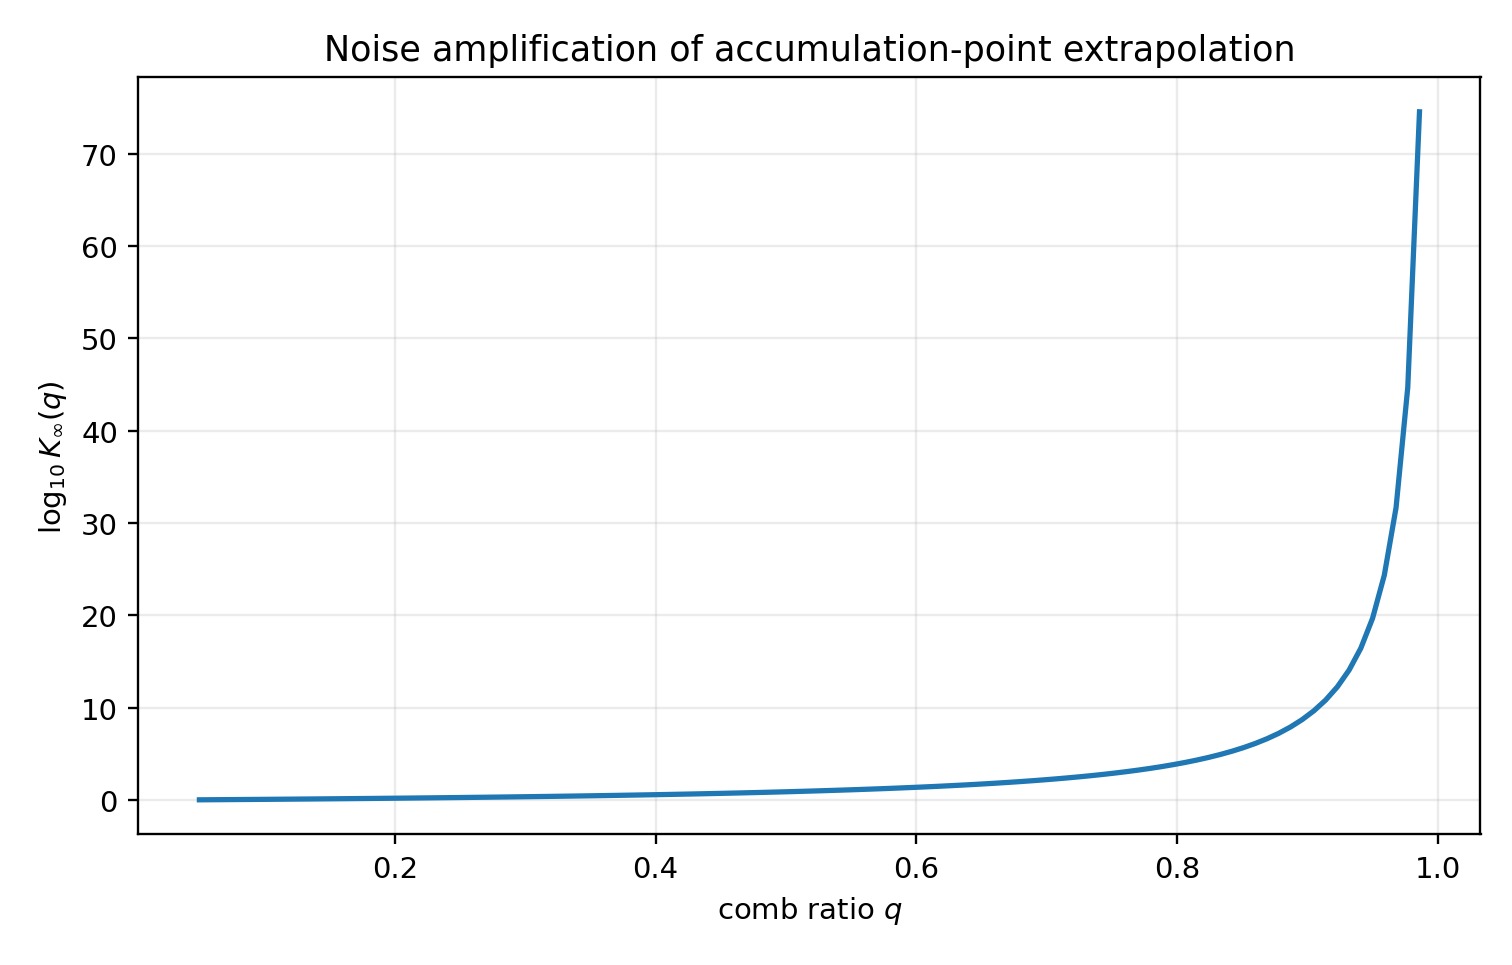
\includegraphics[width=0.88\textwidth]{stability_growth.png}
\caption{The infinite-order total variation
$K_\infty(q)=(-q;q)_\infty/(q;q)_\infty$.  The vertical axis is logarithmic in
base $10$.  Stability is excellent for small and moderate $q$ but deteriorates
nonperturbatively as $q\uparrow1$.}
\label{fig:stability}
\end{figure}

The data file also compares $K_\infty(e^{-t})$ to the asymptotic
\eqref{eq:K-modular}.  For the plotted near-one values the relative difference
is already below the displayed precision, reflecting the exponentially small
modular correction.

\subsection{Regular-variation constants}

\begin{figure}[htbp]
\centering
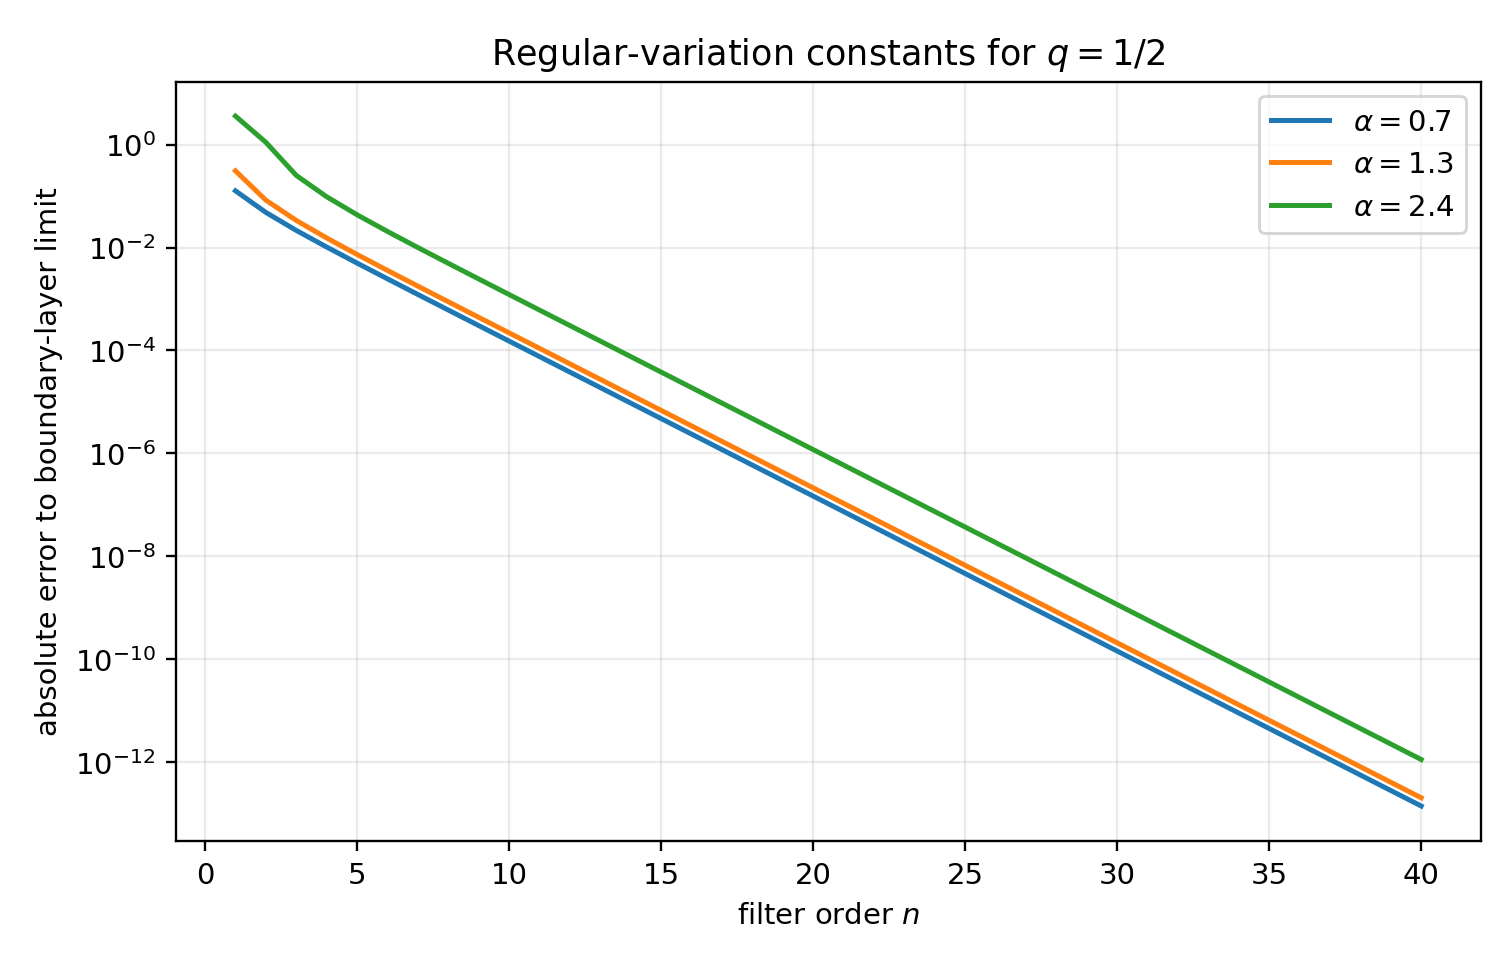
\includegraphics[width=0.88\textwidth]{regular_variation_convergence.png}
\caption{For pure powers $x^\alpha$ at $q=1/2$, the normalized exact multiplier
$(q^{1-\alpha};q)_n/(q;q)_n$ converges geometrically to
$C_q(\alpha)$.  The three exponents illustrate positive and negative limiting
constants.}
\label{fig:regular-variation}
\end{figure}

For example,
\begin{align*}
 C_{1/2}(0.7)&\approx 0.2493175488440439431,\\
 C_{1/2}(1.3)&\approx-0.1538705960439442305,\\
 C_{1/2}(2.4)&\approx 0.2913748265379615867.
\end{align*}
At positive integer exponents the limit is exactly zero, in agreement with
polynomial cancellation.

\subsection{Exact Fabius boundary remainders}

For $A=2^{-(n+1)}$, define
\[
 R_n:=\sum_{k=0}^n\lambda_{n,k}^{(1/2)}F(2^{-(n+1+k)}),
 \qquad
 B_n:=\frac{2^{-n(n+1)}}{(n+1)!}.
\]
The theorem gives $(-1)^nR_n>0$ and $|R_n|/B_n=\Expectation F(S_n)\in(0,1)$.  Exact
fraction arithmetic produces the following decimal summary.

\begin{table}[htbp]
\centering
\caption{Normalized exact dyadic Fabius boundary remainders.}
\label{tab:Fabius-remainders}
\begin{tabular}{rcc}
\toprule
$n$ & sign of $R_n$ & $|R_n|/B_n$\\
\midrule
1  & $-$ & $0.500000000000$\\
2  & $+$ & $0.392067901235$\\
3  & $-$ & $0.285827999336$\\
4  & $+$ & $0.204528650771$\\
5  & $-$ & $0.146778506870$\\
6  & $+$ & $0.106554660592$\\
7  & $-$ & $0.078481279976$\\
8  & $+$ & $0.058671832771$\\
9  & $-$ & $0.044492131277$\\
10 & $+$ & $0.034188031436$\\
\bottomrule
\end{tabular}
\end{table}

\begin{figure}[htbp]
\centering
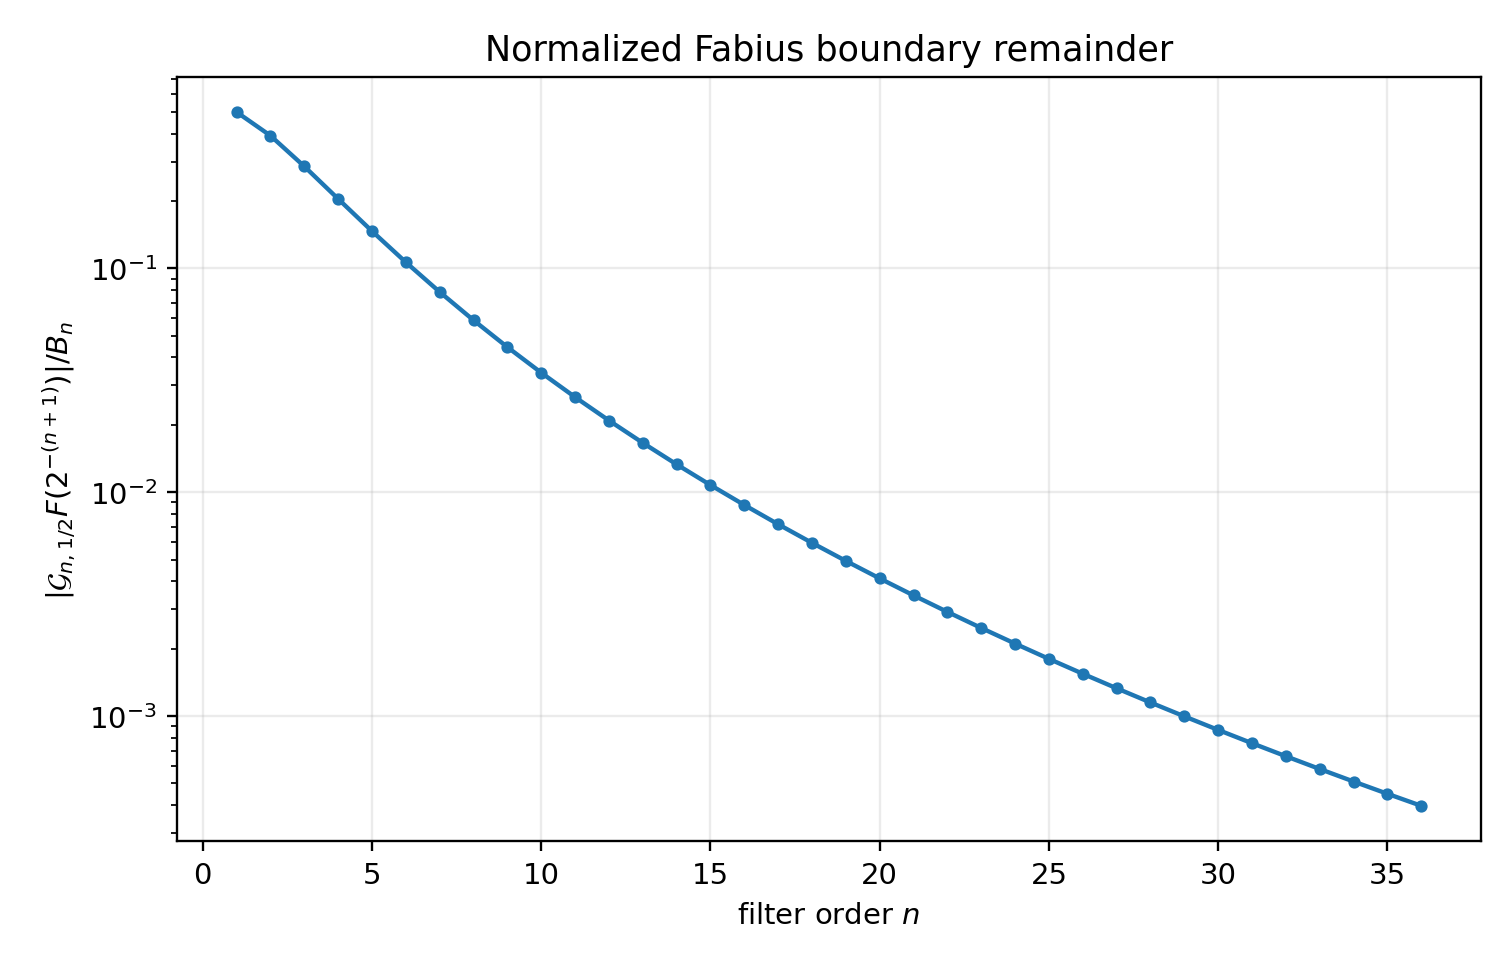
\includegraphics[width=0.88\textwidth]{fabius_boundary_ratio.png}
\caption{The normalized Fabius boundary remainder
$|R_n|/B_n=\Expectation F(S_n)$ through order $36$.  The decrease is much slower than
the already extracted factorial-supergeometric factor $B_n$; its finer
asymptotics are posed as a conjecture in \cref{sec:frontiers}.}
\label{fig:Fabius-ratio}
\end{figure}

\subsection{Reproducibility files}

The script writes four CSV files:
\begin{center}
\begin{tabular}{ll}
\toprule
File & Contents\\
\midrule
\texttt{moment\_checks.csv} & canceled moments and recursion comparison\\
\texttt{stability\_growth.csv} & $K_\infty$, modular approximation, ratio\\
\texttt{regular\_variation.csv} & finite multipliers and limiting constants\\
\texttt{fabius\_boundary.csv} & exact rational filters, bounds, sign checks\\
\bottomrule
\end{tabular}
\end{center}
The archive includes these files and the three PNG figures, so the LaTeX source
can be recompiled without rerunning Python.

\section{Research frontiers and conjectures}
\label{sec:frontiers}

\subsection{A local limit theorem for geometric B-splines}

\cref{eq:Y-scaling-limit} proves weak convergence.  The explicit spline and
limit densities suggest a substantially stronger statement.

\begin{conjecture}[Local density limit]
For every fixed $0<q<1$ and compact interval $K\subset(0,\infty)$,
\begin{equation}
 \sup_{y\in K}
 \left|
 \frac{A}{n+2}B_{n,A,q}\!\left(\frac{Ay}{n+2}\right)-p_q(y)
 \right|\longrightarrow0,
 \label{eq:local-density-conjecture}
\end{equation}
where $p_q$ is given by \eqref{eq:Z-density}.  The convergence should extend to
all derivatives on compact subsets of $(0,\infty)$ after the natural scaling.
\end{conjecture}

A proof might combine the exponential/Dirichlet representation with Fourier or
Laplace inversion and uniform control of the denominator
$(E_*+\cdots+E_n)/(n+2)$.  Such a theorem would turn finite interpolation
kernels into quantitative approximations of a canonical $q$-exponential
density.

\subsection{Fabius--Dirichlet small-value asymptotics}

Let
\[
 \rho_n:=\Expectation F(S_n)=\frac{|R_n|}{B_n}.
\]
The scaling limit $(n+2)S_n\Rightarrow Z_{1/2}$ suggests that $S_n$ is of order
$1/n$, while the Fabius function has a logarithmic-square flatness scale at
zero.  Random fluctuations of $Z_{1/2}$ should affect lower-order terms but not
the leading quadratic logarithm.

\begin{conjecture}[Leading decay of the normalized Fabius remainder]
\begin{equation}
 \log\rho_n
 \sim-\frac{(\log n)^2}{2\log2}
 \qquad(n\to\infty).
 \label{eq:Fabius-rho-conjecture}
\end{equation}
More precisely, the next terms should be obtainable by combining the sharp
Lambert-$W$ endpoint expansion of $F$ developed elsewhere in the ProveIt
project with the density \eqref{eq:Z-density} and a Laplace saddle point.
\end{conjecture}

The experiment in \cref{fig:Fabius-ratio} is consistent with a slowly
converging logarithmic-square law, but orders below $40$ are far too small to
distinguish the lower-order $\log n\log\log n$ and $\log n$ corrections.

\subsection{Second-order regular variation}

\cref{eq:regular-variation} gives only the first boundary-layer limit.  If
$f(x)=x^\alpha L(x)$ and $L$ belongs to a de Haan second-order class, one should
be able to expand
\[
 \frac{(\Gc_{n,q}f)(A)}{f(Aq^n)}
 =C_q(\alpha)+A_1(Aq^n)C_{q,1}(\alpha,\rho)+o(A_1(Aq^n)),
\]
where $A_1$ is the auxiliary function and the correction constant is a
$q$-Mellin moment of the signed boundary layer $\beta_r^{(q)}$.  This would
provide rigorous error estimators for nonanalytic asymptotic extrapolation.

\begin{problem}[Second-order transfer theorem]
Formulate minimal second-order regular-variation hypotheses and compute the
correction constants explicitly from
$(qz;q)_\infty/(q;q)_\infty$.  Treat the resonant integer cases, where
$C_q(\alpha)=0$, separately; there the correction may become the leading term.
\end{problem}

\subsection{The double-scaling transition $q\uparrow1$, $n\to\infty$}

The fixed-order behavior \eqref{eq:fixed-n-q1} and infinite-order behavior
\eqref{eq:K-modular} do not commute.  A natural transition parameter is
$n(1-q)$ or $nt$ when $q=e^{-t}$.

\begin{problem}[Universal transition kernel]
Determine asymptotics of the row polynomial, its total variation, and the
Peano-kernel density when
\[
 n\to\infty,\qquad t\downarrow0,
 \qquad nt\to\tau\in(0,\infty).
\]
One expects a continuum limit connecting geometric-comb extrapolation to
confluent Hermite/Taylor extrapolation at $A$.  The relevant asymptotics should
involve dilogarithms and a saddle point for finite $q$-products.
\end{problem}

\subsection{Optimal filters under analytic priors}

The Gaussian filter is algebraically unique when exactly $n$ integer modes are
canceled with $n+1$ samples.  With more samples than constraints, stability and
bias can be traded.

\begin{problem}[Minimax geometric extrapolation]
Given $M>n$, choose weights on $A,Aq,\ldots,Aq^M$ that preserve constants and
annihilate $x,\ldots,x^n$, while minimizing either total variation or the worst
error over an analytic coefficient-majorant class.  Compare the optimizer with
truncated, damped, and least-squares modifications of $W_{n,q}$.
\end{problem}

The problem is finite-dimensional and convex for total variation, but its
large-$M,n$ structure is likely governed by weighted extremal polynomials on
the spectral set $\{q^m:m\ge0\}$.

\subsection{Inverse Fabius and nonlinear combs}

The inverse Fabius function has endpoint behavior governed by asymptotic
inversion and Lambert $W$, not a regular Taylor series.  A promising strategy is
to choose a nonlinear sample comb $x_k$ so that the dominant inverse asymptotic
modes become geometric in a transformed coordinate.  Confluent modal filters
from \cref{sec:modal} can then remove the leading Lambert-$W$ transseries terms.

\begin{problem}[Lambert-adapted Newton coordinates]
Find a coordinate $u=u(x)$ in which the inverse Fabius germ admits an expansion
in modes $e^{-\alpha u}u^s$, construct the corresponding geometric Newton
series, and determine whether its interpolation coefficients have a positive
kernel or a controlled boundary layer analogous to \eqref{eq:beta}.
\end{problem}

\subsection{Multivariate geometric combs}

Tensor products immediately give interpolation on
$\{A_1q_1^{k_1}\}\times\cdots\times\{A_dq_d^{k_d}\}$, with products of
Gaussian rows.  More interesting are diagonal or simplex combs with a shared
scale index, which interact with multivariate self-similar distributions and
box splines.  The Dirichlet-average interpretation suggests that multivariate
Peano kernels may again have positive probabilistic representations.

\subsection{Formalization boundary and remaining roadmap}

The live Lean corpus has moved beyond a roadmap for the elementary finite
filter.  The modules \nolinkurl{FiniteQBinomialCore.lean},
\nolinkurl{GeometricLagrangeQBinomial.lean},
\nolinkurl{GeometricLagrangeQMoments.lean}, and
\nolinkurl{GeometricLagrangeCompleteHomogeneous.lean} contain named theorems
for finite $q$-products, Gaussian weights, cancellation/residual formulas, the
complete-homogeneous specialization, and the exact finite row norm.
\nolinkurl{LimitConditionNumber.lean} supplies the fixed-$q$ infinite-product
limit, while the geometric-uniform and Rvachev modules named in the opening
status box cover related probability and Fourier infrastructure.

The report-specific obligations that remain are therefore narrower:
\begin{enumerate}[leftmargin=2em]
\item identify geometric divided differences with iterated Jackson derivatives
under explicit field and differentiability hypotheses;
\item construct the infinite Newton series and prove its local uniform
convergence;
\item formalize confluent spectral zeros and the Puiseux--log remainder bound;
\item prove the reversed-row $\ell^1$ limit and the regular-variation transfer;
\item add Hermite--Genocchi/Dirichlet-average infrastructure, the geometric-knot
B-spline moments, and the perpetuity scaling limit;
\item derive the Fabius boundary expectation and the entire scale-reconstruction
theorem from the already formalized finite core.
\end{enumerate}
Until those items exist as checked declarations, the correspondingly labelled
results here remain manuscript theorems.

\section{Conclusions}

Interpolation on a geometric comb is best understood through four mutually
reinforcing representations.

First, it is ordinary Lagrange/Newton interpolation with unusually explicit
products.  Second, it is Jackson calculus: divided differences are normalized
$q$-derivatives, and basis changes are Gaussian-binomial transforms.  Third, it
is a spectral filter for dilation, making power, fractional-power, and
logarithmic asymptotic modes transparent.  Fourth, its smooth remainder is a
positive B-spline/Dirichlet average whose moments and scaling limit are
$q$-products.

These representations clarify the Fabius/Rvachev connection.  Geometrically
weighted uniforms produce finite box splines and, at the dyadic value,
Thue--Morse coefficients.  The Fabius endpoint differential equation converts
the Peano remainder into an exact positive expectation with alternating outer
sign.  The Rvachev Fourier transform is even, so physical scaling by $c$ becomes
geometric interpolation with base $c^2$; at $c=1/2$ this improves the stability
constant from about $8.26$ to about $1.97$.

The theory also separates two facts that can otherwise be confused.  The
Vandermonde coefficient problem is severely ill conditioned, but the
accumulation-point functional is uniformly stable for fixed $q<1$.  The reason
is a universal signed boundary layer concentrated at the smallest samples.
That boundary layer controls continuous convergence and regularly varying
asymptotics, while the positive Peano kernel controls smooth signs and
factorial error bounds.

The resulting framework is broad enough to support modal extrapolation,
Fabius endpoint analysis, Fourier moment filters, and future work on inverse
functions and double-scaling limits, yet concrete enough for exact rational
computation and formal proof.

\appendix

\section{Additional derivations}

\subsection{Partial fractions for the $q$-exponential perpetuity}

For completeness, consider
\[
 L_q(s)=\prod_{j=0}^{\infty}(1+sq^j)^{-1}.
\]
At the simple pole $s=-q^{-k}$, the coefficient of
$(1+sq^k)^{-1}$ is
\begin{align*}
 c_k
 &=\left[\prod_{j\ne k}(1-q^{j-k})\right]^{-1}\\
 &=\frac{(-1)^kq^{k(k+1)/2}}{(q;q)_k(q;q)_\infty}.
\end{align*}
Indeed, the factors with $j<k$ give
$(-1)^kq^{-k(k+1)/2}(q;q)_k$, and the factors with $j>k$ give
$(q;q)_\infty$.  Since
\[
 \mathcal L^{-1}\left[\frac1{1+sq^k}\right](y)
 =q^{-k}e^{-y/q^k},
\]
we recover \eqref{eq:Z-density}.

\subsection{Equivalence of the power formulas}

For an integer $d=n+1+r$, \eqref{eq:pure-power} and
\eqref{eq:all-moments} agree.  Indeed,
\begin{align*}
 q^{dn}\frac{(q^{1-d};q)_n}{(q;q)_n}
 &=q^{(n+1+r)n}
 \frac{\prod_{j=0}^{n-1}(1-q^{-n-r+j})}{(q;q)_n}\\
 &=(-1)^nq^{\binom{n+1}{2}}
 \frac{(q;q)_{n+r}}{(q;q)_n(q;q)_r}\\
 &=(-1)^nq^{\binom{n+1}{2}}\GaussianBinomial{n+r}{n}{q}.
\end{align*}
This calculation is often useful when moving between Mellin exponents and
integer Taylor moments.

\subsection{A generating function for the smooth remainder on exponentials}

Take $f(x)=e^{tx}$ in \eqref{eq:HG-remainder}.  Using
\eqref{eq:Y-moments},
\begin{align}
 (\Gc_{n,q}e^{t\cdot})(A)-1
 &=\frac{(-1)^nA^{n+1}q^{\binom{n+1}{2}}t^{n+1}}{(n+1)!}
 \Expectation e^{tY_{n,A,q}}\notag\\
 &=(-1)^nA^{n+1}q^{\binom{n+1}{2}}t^{n+1}
 \sum_{r=0}^{\infty}
 \frac{A^r\GaussianBinomial{n+r}{n}{q}}{(n+r+1)!}t^r.
 \label{eq:exp-remainder}
\end{align}
The same series follows from \eqref{eq:exact-analytic-tail}.  The equality is a
useful consistency check between the analytic-tail and B-spline pictures.

\section{Companion-code notes}

The Python source intentionally avoids black-box interpolation routines.  Every
quantity is implemented from the formulas proved in the report.  The key
functions are:
\begin{description}[leftmargin=3.6cm,style=nextline]
\item[\texttt{origin\_lagrange\_weights}]
implements \eqref{eq:lambda};
\item[\texttt{recursive\_filter}]
implements \eqref{eq:triangular-filter};
\item[\texttt{stability\_factor\_infinite}]
computes \eqref{eq:K-infinity};
\item[\texttt{regular\_variation\_constant}]
computes \eqref{eq:regular-variation};
\item[\texttt{fabius\_dyadic\_values\_exact}]
implements \eqref{eq:V-recurrence} with rational arithmetic;
\item[\texttt{fabius\_boundary\_filter\_exact}]
checks \eqref{eq:F-dyadic-filter} exactly.
\end{description}
The script can be rerun from the archive directory with
\begin{verbatim}
python geometric_comb_experiments.py
\end{verbatim}
It overwrites only the listed CSV and PNG outputs.

\begin{thebibliography}{99}

\bibitem{AnnabyMansour}
M.~H. Annaby and Z.~S. Mansour,
\newblock $q$-Taylor and interpolation series for Jackson $q$-difference
operators,
\newblock \emph{Journal of Mathematical Analysis and Applications} 344 (2008),
472--483,
\newblock doi:10.1016/j.jmaa.2008.02.033.

\bibitem{AriasDeReyna}
J. Arias de Reyna,
\newblock An infinitely differentiable function with compact support:
definition and properties,
\newblock \emph{Revista de la Real Academia de Ciencias Exactas, Fisicas y
Naturales de Madrid} 76 (1982), 21--38;
\newblock reprint arXiv:1702.05442.

\bibitem{BinghamGoldieTeugels}
N.~H. Bingham, C.~M. Goldie, and J.~L. Teugels,
\newblock \emph{Regular Variation},
\newblock Cambridge University Press, 1987.

\bibitem{CurrySchoenberg}
H.~B. Curry and I.~J. Schoenberg,
\newblock On Polya frequency functions IV: the fundamental spline functions
and their limits,
\newblock \emph{Journal d'Analyse Mathematique} 17 (1966), 71--107.

\bibitem{deBoor}
C. de Boor,
\newblock \emph{A Practical Guide to Splines}, revised edition,
\newblock Springer, 2001.

\bibitem{DLMF17}
NIST Digital Library of Mathematical Functions,
\newblock Chapter 17: $q$-Hypergeometric and Related Functions,
\newblock \url{https://dlmf.nist.gov/17}, accessed 30 August 2026.

\bibitem{Fabius1966}
J. Fabius,
\newblock A probabilistic example of a nowhere analytic $C^\infty$-function,
\newblock \emph{Zeitschrift fur Wahrscheinlichkeitstheorie und Verwandte
Gebiete} 5 (1966), 173--174,
\newblock doi:10.1007/BF00536652.

\bibitem{GasperRahman}
G. Gasper and M. Rahman,
\newblock \emph{Basic Hypergeometric Series}, second edition,
\newblock Cambridge University Press, 2004.

\bibitem{Ismail}
M.~E.~H. Ismail,
\newblock \emph{Classical and Quantum Orthogonal Polynomials in One Variable},
\newblock Cambridge University Press, 2005.

\bibitem{KacCheung}
V. Kac and P. Cheung,
\newblock \emph{Quantum Calculus},
\newblock Springer, 2002.

\bibitem{ProveItFabius}
V. Reshetnikov,
\newblock Primary semi-formalized exposition on the Fabius and Rvachev
functions,
\newblock ProveIt repository, directory
\texttt{Analysis/FabiusFunction/docs},
\newblock \url{https://github.com/VladimirReshetnikov/ProveIt},
accessed 30 August 2026.

\bibitem{ProveItMonograph}
V. Reshetnikov,
\newblock \emph{$q$-Pochhammer symbols and $q$-binomial coefficients: a
semi-formalized monograph},
\newblock ProveIt repository,
\newblock \url{https://github.com/VladimirReshetnikov/ProveIt/blob/main/Analysis/FabiusFunction/docs/semi-formalized-research-frontiers/drafts/exponents-and-q-series/q_pochhammer_q_binomial_monograph/q_pochhammer_q_binomial_monograph.tex},
accessed 30 August 2026.

\bibitem{Rvachev1990}
V.~A. Rvachev,
\newblock Compactly supported solutions of functional-differential equations
and their applications,
\newblock \emph{Russian Mathematical Surveys} 45:1 (1990), 87--120,
\newblock doi:10.1070/RM1990v045n01ABEH002324.

\bibitem{SimeonovGoldman}
P. Simeonov and R. Goldman,
\newblock Quantum B-splines,
\newblock \emph{BIT Numerical Mathematics} 53 (2013), 193--223,
\newblock doi:10.1007/s10543-012-0395-z.

\end{thebibliography}

\end{document}
